% Tech Science Press TSP-template migration of cas-dc-sample-rev2-SI.tex
% TARGET JOURNAL: Computers, Materials & Continua (CMC).
% rev5: references moved to references.bib (BibTeX); abstract abbreviations that
% occur only once are now written out, per the CMC Instructions for Authors.
% Submit LaTeX as ONE zip containing this file, Definitions/, references.bib,
% netmodel.pdf, and any .bst you point \bibliographystyle at.
\documentclass[cmc,article,submit,moreauthors,pdftex]{Definitions/tsp}
%%%%Update on 30 November 2023%%%
\usepackage[normalem]{ulem} % For using the command \uuline{} in the \abstract 
\usepackage{amsfonts} % Use for some special math mark
%%\usepackage{pxfonts} % Use for some special math mark 
%\usepackage{wasysym} % Use for some special mark
%\usepackage{subfigure} % For some paper the use \subfigure
\usepackage{mathcomp} % For permille mark
\usepackage{CJKutf8} % For Chinese font
\usepackage{pifont} % For some special mark 
\usepackage{bm} % Forr math enviroment bold format
\usepackage{bbm} % For some math fancy characters
\graphicspath{{./Definitions/}} % Use for import path the figures paper used

\makeatletter
\def\T@n@@nc@d@ngM@cr@M@d{}
\def\LY@n@@nc@d@ngM@cr@M@d{}
\makeatother

\let\orignewcommand\newcommand  % Store the original \newcommand
\let\newcommand\providecommand  % Make \newcommand behave like \providecommand
\usepackage{verse}
\let\newcommand\orignewcommand  % Use the original `\newcommand` in future
\makeatletter
\renewcommand*{\theHpoemline}{\arabic{verse@envctr}.\arabic{poemline}} % Use the original definition from verse.sty
\makeatother

% Define a matrix envrioment
\newsavebox\foobox
\newcommand{\slantbox}[2][.2]{\mbox{%
        \sbox{\foobox}{#2}%
        \hskip\wd\foobox
        \pdfsave
        \pdfsetmatrix{1 0 #1 1}%
        \llap{\usebox{\foobox}}%
        \pdfrestore
}}

%\setlength{\fboxsep}{0cm}

% Define triangledown mark
\let\oldblacktriangledown\blacktriangledown

% Define \dagger using unicode
\renewcommand{\dagger}{\mathchar"2279}
\renewcommand{\ddagger}{\mathchar"227A}

% Define italic In, Max
\newcommand{\mmathit}[1]{
  \ifthenelse{\equal{#1}{\ln}}{\mathit{ln}}{
    \ifthenelse{\equal{#1}{\max}}{\mathit{max}}{\mathit{#1}}
  }
}
\makeatother
\robustify{\footnote}

\DeclareUnicodeCharacter{1E45}{\.{n}}
\DeclareUnicodeCharacter{1E41}{\.{m}}
\DeclareUnicodeCharacter{2003}{\quad}
%\DeclareUnicodeCharacter{0177}{\^{y}}
%\DeclareUnicodeCharacter{101}{\={a}}
\DeclareUnicodeCharacter{2009}{\thinspace}
\DeclareUnicodeCharacter{2002}{\enspace{}}
\DeclareUnicodeCharacter{2005}{\thinspace}
\DeclareUnicodeCharacter{0263}{\textipa{G}}
%\DeclareUnicodeCharacter{117}{\.{e}}
\DeclareUnicodeCharacter{A0}{~}
\DeclareUnicodeCharacter{2460}{\textcircled{\scriptsize{1}}}
\DeclareUnicodeCharacter{2461}{\textcircled{\scriptsize{2}}}
\DeclareUnicodeCharacter{2462}{\textcircled{\scriptsize{3}}}
\DeclareUnicodeCharacter{2463}{\textcircled{\scriptsize{4}}}
\DeclareUnicodeCharacter{2464}{\textcircled{\scriptsize{5}}}
\DeclareUnicodeCharacter{2465}{\textcircled{\scriptsize{6}}}
\DeclareUnicodeCharacter{2466}{\textcircled{\scriptsize{7}}}
\DeclareUnicodeCharacter{2467}{\textcircled{\scriptsize{8}}}
\DeclareUnicodeCharacter{2468}{\textcircled{\scriptsize{9}}}
\DeclareUnicodeCharacter{2070}{\textsuperscript{0}}
\DeclareUnicodeCharacter{2074}{\textsuperscript{4}}
\DeclareUnicodeCharacter{2075}{\textsuperscript{5}}
\DeclareUnicodeCharacter{2076}{\textsuperscript{6}}
\DeclareUnicodeCharacter{2077}{\textsuperscript{7}}
\DeclareUnicodeCharacter{2078}{\textsuperscript{8}}
\DeclareUnicodeCharacter{2079}{\textsuperscript{9}}
\DeclareUnicodeCharacter{02C2}{<}
\DeclareUnicodeCharacter{2033}{\relax\ifmmode '' \else $''$\fi}
\DeclareUnicodeCharacter{2034}{\relax\ifmmode ''' \else $'''$\fi}
\DeclareUnicodeCharacter{2026}{\relax\ifmmode … \else $\ldots$\fi}
\DeclareUnicodeCharacter{0229}{\c{e}}
\DeclareUnicodeCharacter{016F}{\r{u}}
%\DeclareUnicodeCharacter{0218}{\cb{S}}
%\DeclareUnicodeCharacter{0219}{\cb{s}}
%\DeclareUnicodeCharacter{021B}{\cb{t}}
\DeclareUnicodeCharacter{127}{\relax\ifmmode\rm\hbar\else $\rm\hbar$\fi}
\DeclareUnicodeCharacter{3AC}{\relax\ifmmode\acute{\alpha}\else $\acute{\alpha}$\fi}
\DeclareUnicodeCharacter{3AD}{\relax\ifmmode\acute{\varepsilon}\else $\acute{\varepsilon}$\fi}
\DeclareUnicodeCharacter{3AE}{\relax\ifmmode\acute{\eta}\else $\acute{\eta}$\fi}
\DeclareUnicodeCharacter{3AF}{\relax\ifmmode\acute{\iota}\else $\acute{\iota}$\fi}
\DeclareUnicodeCharacter{3CC}{\relax\ifmmode\acute{o}\else $\acute{o}$\fi}
\DeclareUnicodeCharacter{3CD}{\relax\ifmmode\acute{\upsilon}\else $\acute{\upsilon}$\fi}
\DeclareUnicodeCharacter{3CE}{\relax\ifmmode\acute{\omega}\else $\acute{\omega}$\fi}
\DeclareUnicodeCharacter{391}{A}
\DeclareUnicodeCharacter{392}{B}
\DeclareUnicodeCharacter{395}{E}
\DeclareUnicodeCharacter{396}{Z}
\DeclareUnicodeCharacter{397}{H}
\DeclareUnicodeCharacter{399}{I}
\DeclareUnicodeCharacter{39A}{K}
\DeclareUnicodeCharacter{39C}{M}
\DeclareUnicodeCharacter{39D}{N}
\DeclareUnicodeCharacter{39F}{O}
\DeclareUnicodeCharacter{3A1}{P}
\DeclareUnicodeCharacter{3A4}{T}
\DeclareUnicodeCharacter{3A7}{X}

\DeclareUnicodeCharacter{27E6}{\relax\ifmmode \llbracket \else $\llbracket$\fi}
\DeclareUnicodeCharacter{27E7}{\relax\ifmmode \rrbracket \else $\rrbracket$\fi}
\DeclareUnicodeCharacter{00B5}{\relax\ifmmode \mu{} \else $\mu$\fi}
\DeclareUnicodeCharacter{1D434}{\relax\ifmmode A \else $A$\fi}
\DeclareUnicodeCharacter{1D435}{\relax\ifmmode B \else $B$\fi}
\DeclareUnicodeCharacter{1D436}{\relax\ifmmode C \else $C$\fi}
\DeclareUnicodeCharacter{1D437}{\relax\ifmmode D \else $D$\fi}
\DeclareUnicodeCharacter{1D438}{\relax\ifmmode E \else $E$\fi}
\DeclareUnicodeCharacter{1D439}{\relax\ifmmode F \else $F$\fi}
\DeclareUnicodeCharacter{1D43A}{\relax\ifmmode G \else $G$\fi}
\DeclareUnicodeCharacter{1D43B}{\relax\ifmmode H \else $H$\fi}
\DeclareUnicodeCharacter{1D43C}{\relax\ifmmode I \else $I$\fi}
\DeclareUnicodeCharacter{1D43D}{\relax\ifmmode J \else $J$\fi}
\DeclareUnicodeCharacter{1D43E}{\relax\ifmmode K \else $K$\fi}
\DeclareUnicodeCharacter{1D43F}{\relax\ifmmode L \else $L$\fi}
\DeclareUnicodeCharacter{1D440}{\relax\ifmmode M \else $M$\fi}
\DeclareUnicodeCharacter{1D441}{\relax\ifmmode N \else $N$\fi}
\DeclareUnicodeCharacter{1D442}{\relax\ifmmode O \else $O$\fi}
\DeclareUnicodeCharacter{1D443}{\relax\ifmmode P \else $P$\fi}
\DeclareUnicodeCharacter{1D444}{\relax\ifmmode Q \else $Q$\fi}
\DeclareUnicodeCharacter{1D445}{\relax\ifmmode R \else $R$\fi}
\DeclareUnicodeCharacter{1D446}{\relax\ifmmode S \else $S$\fi}
\DeclareUnicodeCharacter{1D447}{\relax\ifmmode T \else $T$\fi}
\DeclareUnicodeCharacter{1D448}{\relax\ifmmode U \else $U$\fi}
\DeclareUnicodeCharacter{1D449}{\relax\ifmmode V \else $V$\fi}
\DeclareUnicodeCharacter{1D44A}{\relax\ifmmode W \else $W$\fi}
\DeclareUnicodeCharacter{1D44B}{\relax\ifmmode X \else $X$\fi}
\DeclareUnicodeCharacter{1D44C}{\relax\ifmmode Y \else $Y$\fi}
\DeclareUnicodeCharacter{1D44D}{\relax\ifmmode Z \else $Z$\fi}
\DeclareUnicodeCharacter{1D44E}{\relax\ifmmode a \else $a$\fi}
\DeclareUnicodeCharacter{1D44F}{\relax\ifmmode b \else $b$\fi}
\DeclareUnicodeCharacter{1D450}{\relax\ifmmode c \else $c$\fi}
\DeclareUnicodeCharacter{1D451}{\relax\ifmmode d \else $d$\fi}
\DeclareUnicodeCharacter{1D452}{\relax\ifmmode e \else $e$\fi}
\DeclareUnicodeCharacter{1D453}{\relax\ifmmode f \else $f$\fi}
\DeclareUnicodeCharacter{1D454}{\relax\ifmmode g \else $g$\fi}
\DeclareUnicodeCharacter{1D456}{\relax\ifmmode i \else $i$\fi}
\DeclareUnicodeCharacter{1D457}{\relax\ifmmode j \else $j$\fi}
\DeclareUnicodeCharacter{1D458}{\relax\ifmmode k \else $k$\fi}
\DeclareUnicodeCharacter{1D459}{\relax\ifmmode l \else $l$\fi}
\DeclareUnicodeCharacter{1D45A}{\relax\ifmmode m \else $m$\fi}
\DeclareUnicodeCharacter{1D45B}{\relax\ifmmode n \else $n$\fi}
\DeclareUnicodeCharacter{1D45C}{\relax\ifmmode o \else $o$\fi}
\DeclareUnicodeCharacter{1D45D}{\relax\ifmmode p \else $p$\fi}
\DeclareUnicodeCharacter{1D45E}{\relax\ifmmode q \else $q$\fi}
\DeclareUnicodeCharacter{1D45F}{\relax\ifmmode r \else $r$\fi}
\DeclareUnicodeCharacter{1D460}{\relax\ifmmode s \else $s$\fi}
\DeclareUnicodeCharacter{1D461}{\relax\ifmmode t \else $t$\fi}
\DeclareUnicodeCharacter{1D462}{\relax\ifmmode u \else $u$\fi}
\DeclareUnicodeCharacter{1D463}{\relax\ifmmode v \else $v$\fi}
\DeclareUnicodeCharacter{1D464}{\relax\ifmmode w \else $w$\fi}
\DeclareUnicodeCharacter{1D465}{\relax\ifmmode x \else $x$\fi}
\DeclareUnicodeCharacter{1D466}{\relax\ifmmode y \else $y$\fi}
\DeclareUnicodeCharacter{1D467}{\relax\ifmmode z \else $z$\fi}

\DeclareUnicodeCharacter{1E67}{\.{\v s}}
\DeclareUnicodeCharacter{1E11}{\relax\ifmmode \c{d} \else $\c{d}$\fi}
\DeclareUnicodeCharacter{1ECB}{\relax\ifmmode \d{i} \else $\d{i}$\fi}
\DeclareUnicodeCharacter{1D8D}{\relax\ifmmode \textlhookx \else $\textlhookx$\fi}
\DeclareUnicodeCharacter{104}{\relax\ifmmode \k{A} \else $\k{A}$\fi}
\DeclareUnicodeCharacter{211E}{\relax\ifmmode \textrecipe \else $\textrecipe$\fi}
\DeclareUnicodeCharacter{29D}{\relax\ifmmode \textctj \else $\textctj$\fi}

\DeclareUnicodeCharacter{1E2E}{\'{\"I}}
\DeclareUnicodeCharacter{23F}{\textrts}

\DeclareUnicodeCharacter{2C73}{\varw}

\DeclareUnicodeCharacter{2127}{\mho}

\DeclareUnicodeCharacter{28C}{\textturnv}
\DeclareUnicodeCharacter{252}{\textturnscripta}
\DeclareUnicodeCharacter{259}{\schwa}
\DeclareUnicodeCharacter{25B}{\m{e}}
\DeclareUnicodeCharacter{266}{\m{h}}
\DeclareUnicodeCharacter{127}{\B{h}}
\DeclareUnicodeCharacter{27E}{\textfishhookr}
\DeclareUnicodeCharacter{281}{\textinvscr}


\pdfminorversion=7

\continuouspages{}
\firstpage{1}
\makeatletter
\setcounter{page}{\@firstpage}
\makeatother
\pubvolume{0}
\issuenum{0}
\elocationid{0}
\articlenumber{}
\pubyear{2026}
\copyrightyear{2026}
\datereceived{}
\dateaccepted{}
\dateonlinefirst{}
\datepublished{}
\doinum{}

\newcolumntype{Y}{>{\centering\arraybackslash}X}
\setlength{\headheight}{38.3pt}
% Keep the protocol notation within pdfTeX's math-alphabet limit of the TSP font setup.
\renewcommand{\mathsf}[1]{\mathrm{#1}}
\renewcommand{\mathcal}[1]{\mathrm{#1}}
\renewcommand{\mathbb}[1]{\mathrm{#1}}

% Protocol notation and ROR macros
\newcommand{\cc}{\mathbin{\|}}
\newcommand{\CT}{\mathsf{CT}}
\newcommand{\Gen}{\mathrm{Gen}}
\newcommand{\Rep}{\mathrm{Rep}}
\newcommand{\advA}{\mathcal{A}}

% The article has no assigned DOI at submission; retain the TSP title block but suppress its provisional DOI line.
\makeatletter
\renewcommand{\@maketitle}{%
\noindent\rule{0pt}{1.3cm}\par
\begin{flushleft}
  \vspace{-1cm}
  \fontsize{9}{9}\selectfont
  {\boldmath\bfseries{\underline{\@arttype}}}\par
  \vspace{18pt}
  \fontsize{14}{16}\selectfont
  \boldmath\bfseries{\@Title}\par
  \vspace{18pt}
  \fontsize{11}{11}\selectfont
  \boldmath\bfseries{\@Author}\par
  \vspace{6pt}
\end{flushleft}%
}
\makeatother

\Title{A Lightweight Four-Credential Authentication and Key Agreement Protocol for AI-Enabled Edge-IIoT: Transcript-Bound Resistance to Replay and Impersonation}
\TitleCitation{Lightweight Four-Credential Authentication and Key Agreement for AI-Enabled Edge-IIoT}
\Author{Xun Zhang\textsuperscript{1}, Zhiying Mu\textsuperscript{1,*}, Wu Wei\textsuperscript{1}, Zhihui Mu\textsuperscript{1}, Dejun Mu\textsuperscript{1} and Xin Liu\textsuperscript{2}}
% Distinguish the two authors whose family name and first initial are both Mu Z.
\AuthorCitation{Zhang X, Mu ZY, Wei W, Mu ZH, Mu D and Liu X}
\AuthorNames{Xun Zhang, Zhiying Mu, Wu Wei, Zhihui Mu, Dejun Mu and Xin Liu}

\address{%
\textsuperscript{1}School of Cyberspace Security, Northwestern Polytechnical University, Xi'an 710072, China

\textsuperscript{2}School of Artificial Intelligence, Lanzhou University, Lanzhou 730000, China
}

\corres{Corresponding Author: Zhiying Mu. Email: muzhiying@mail.nwpu.edu.cn}

\abstract{Edge intelligence places model inference and data aggregation on edge nodes deployed outside tightly controlled premises. The edge node therefore decides who may query a deployed model and whose measurements may reach its input. We present an authentication and key agreement scheme using a password, smart card, biometric, and Cognitively Evaluable Authentication Factor (CEAF). CEAF is a session-dependent knowledge credential derived from a fresh challenge and checked against edge-side state. The hash--XOR exchange uses nonces and timestamps, while version-bound two-record state tolerates one lost authentication message without re-registration. The ROR analysis separates password and biometric guessing, transcript collisions, forgery, and CEAF-response enumeration. Sensitivity analysis shows how the residual guessing probability changes with the segment count and the admitted-attempt budget. The main protocol provides session-key independence but neither perfect forward secrecy nor key opacity from the edge node. The analytical unit-cost estimate is $0.4588$\,ms; a host reference implementation measured $0.0226$\,ms for the summed software roles on an AMD Ryzen 7 7800X3D, excluding communication and I/O. The construction is a pre-inference access-control mechanism for edge-intelligent IIoT, not a model-level defense. In particular, because $Q_1$ is a transcript-bound hash, exposure of the smart card, password, and biometric permits offline enumeration of the CEAF response from a recorded login; the scheme does not claim offline resistance under that compromise.}
\keyword{security guardrails for AI systems; AI-enabled Industrial Internet of Things; edge intelligence; pre-inference access control; authentication and key agreement; automated credential attacks}

% ===================== rev6 compression additions =====================
% Vertical-space and table-density tightening. If Definitions/package already
% loads enumitem/etoolbox/adjustbox, the no-option \usepackage lines below are
% harmless (LaTeX ignores a re-load without new options).
\usepackage{enumitem}
\usepackage{etoolbox}
\setlist{nosep,leftmargin=1.5em}
\AtBeginEnvironment{tabularx}{\footnotesize}
\setlength{\tabcolsep}{4pt}
\renewcommand{\arraystretch}{0.88}
\setlength{\textfloatsep}{6pt plus 2pt minus 2pt}
\setlength{\floatsep}{4pt plus 1pt minus 1pt}
\setlength{\intextsep}{5pt plus 1pt minus 1pt}
\setlength{\abovedisplayskip}{4pt plus 1pt minus 1pt}
\setlength{\belowdisplayskip}{4pt plus 1pt minus 1pt}
\setlength{\abovedisplayshortskip}{2pt plus 1pt}
\setlength{\belowdisplayshortskip}{2pt plus 1pt}
% Low-vertical-space centred-display environment replacing bare center wrappers.
% Protocol displays receive a visible P-number; the analytical bounds below use
% ordinary equation numbers (1)--(3).
\newcounter{protoeq}
\newenvironment{ceq}{%
  \refstepcounter{protoeq}%
  \par\vspace{-3pt}\setlength{\topsep}{0pt}\setlength{\partopsep}{0pt}\begin{center}%
}{%
  \hspace{0.45em}\textup{(P\theprotoeq)}%
  \end{center}\vspace{-3pt}%
}
% Compact the reference list without changing the main-text typography.
\AtBeginEnvironment{thebibliography}{%
  \fontsize{6.5}{6.5}\selectfont
  \setlength{\itemsep}{-0.3pt}%
  \setlength{\parsep}{0pt}%
}
% The class resets the bibliography font inside \thebibliography; patch that
% reset so the compact reference setting is actually applied.
\makeatletter
\patchcmd{\thebibliography}{\fontsize{10}{11}\selectfont}{\fontsize{6.5}{6.5}\selectfont}{}{}
\makeatother
% ======================================================================

\begin{document}


\section{Introduction}

The convergence of the Internet of Things and cyber-physical systems has made IIoT networks responsible for time-sensitive monitoring and control. Sending all sensor data to a remote cloud adds delay, bandwidth contention, and exposure of operational data \cite{shi}. Edge computing moves computation and storage closer to the source \cite{ranaweera}. It also hosts learned models for anomaly detection, predictive maintenance, and visual inspection. The ``user--edge node--sensor node'' architecture therefore describes an edge-intelligent system: the edge node authenticates users, aggregates sensor data, relays traffic, and serves local model queries.

This setting inherits the security and privacy challenges of resource-constrained and physically accessible wireless-sensor deployments \cite{jabbari,wu2017privacy}. Once the edge node hosts inference, a failed access decision can expose model queries or admit fabricated model inputs. Authentication is therefore the outermost guardrail and must precede model-level defenses. An AKA protocol for this environment must authenticate all three parties, establish a user--sensor key, preserve endpoint anonymity on the channel, and resist replay, modification, impersonation, and man-in-the-middle attacks \cite{wang2021revisit,singh}; related lightweight constructions make the same requirements explicit \cite{shuai,rangwani}. We treat the TEE-protected edge node as a trusted intermediary and state this assumption explicitly in Sections~\ref{sec:threat} and~\ref{sec:conclusions}.

Static passwords remain vulnerable to low-entropy choice, reuse, leakage, keylogging, and observation even when a card or biometric is added \cite{basharzad,liu2019robust,shakirov}; related analyses report the same exposure in deployed authentication systems \cite{khalid}. Learned password models increase the rate of offline guesses \cite{hitaj2019passgan,xu2023passbert}; phishing and credential stuffing extend the same exposure to large-scale attempts. Work performed on the attacker's own hardware is outside a defender-controlled rate limit, so protocols that rely on static credentials inherit this exposure.

A dynamic credential can reduce replay and single-observation exposure by making the accepted response session dependent \cite{kong}. Conventional dynamic-password or OTP designs typically require a token or repeated secret entry; local-verifier variants place additional verification material on the login device. CEAF keeps its verifier at $EN$ and asks the user to select one candidate per segment from a fresh challenge. Unlike a fixed indexed PIN, randomized candidate positions do not expose a permanent index-to-response mapping; unlike a token-based OTP, CEAF needs no additional hardware; unlike a full manual dynamic password, it reduces the calculation to one selection per segment. At $s=3$ this is three selections rather than $21$ manual shifts, but randomized display, lighting, training, and observation affect human error and shoulder-surfing risk; no empirical error rate is claimed. The response must still be bound to the current transcript, and live requests remain subject to source/global controls. A recorded $Q_1$ remains an offline test when the other credentials are exposed.

Existing constructions usually satisfy only part of this objective. Dynamic-password schemes for WSNs and health-record access do not directly model an edge intermediary \cite{yusuf,chen,turkanovic2013}. Other multi-factor and edge-oriented constructions make related trade-offs \cite{amin,li2018threefactor,li2018ecc}. Xu et al. use ECC \cite{xu}; Cui et al. use group signatures and proxy re-encryption \cite{cui}; and Shang et al. use hashes and XOR \cite{shang}. The design gap is a user-generated response that is dynamic, transcript-bound, and inexpensive for constrained devices. The present construction addresses that gap while treating offline CEAF enumeration after multi-credential compromise as an explicit limitation.

We introduce a Cognitively Evaluable Authentication Factor (CEAF) and build a four-credential AKA scheme around it. A fresh challenge and a memorized, evolving secret determine each response. The login device displays candidates and collects the user's choice; the first-message authenticator binds that response to the transcript. Here, a \emph{credential} means one provisioned secret or evidence item that can be compromised and accounted for separately. Password and CEAF are both knowledge credentials, while the smart card represents possession and the biometric represents inherence; therefore ``four-credential'' does not assert four statistically independent factor categories. The term describes the four independently provisioned inputs used by the protocol, not a claim that the scheme supplies four classical factor classes.

The construction is deliberately non-learning: no classifier or learned component appears in the protocol. It supplies the access-control layer for an edge-intelligent deployment and is evaluated as a protocol mechanism, not as a detector.

The mechanism controls admission: which principals may open a session, which sensor may inject measurements, and which requests reach local inference. It does not control the model after an authenticated request is admitted. Prompt injection, training-data or model poisoning, adversarial examples, and model extraction or membership inference are outside the protocol and are discussed in Section~\ref{sec:aisec}. Section~\ref{sec:guardrail} records this boundary. The contributions are:

\begin{enumerate}
\item A segmented cognitive primitive: a response guess succeeds with probability $26^{-s}$, and two consecutive observations recover its state.
\item Edge-side CEAF state and transcript binding, together with source/global ingress limits for live attempts. A recorded $Q_1$ remains an offline test after exposure of the card, password, and biometric; this limitation is included in the security analysis.
\item Two-record state that tolerates one lost message in the four-message authentication exchange, so that a dropped message costs one round of availability instead of forcing re-registration.
\item An ROR bound that separates credential guessing, transcript collisions, forgery, and CEAF-response enumeration, and records the protocol's negative security results.
\end{enumerate}

%%%%%%%%%%%%%%%%%%%%%%%%%%%%%%%%%%%%%%%%%%
\section{Related Work}

Related AKA schemes fall into two architectural stages. Earlier WSN work places a gateway between the user and sensor. Recent edge-IIoT work replaces it with an edge node whose deployment, resources, and trust assumptions differ. The WSN literature still supplies many relevant lightweight authentication ideas.

\subsection{Authentication Schemes in the WSN Stage}

Wong et al. \cite{wong} introduced dynamic authentication for resource-constrained WSNs. Das \cite{das} developed an early two-factor scheme; Paliwal \cite{paliwal} studied authentication for industrial sensing. Turkanovi\'c and H\"olbl \cite{turkanovic2013} developed a dynamic-password construction later extended to heterogeneous IoT deployments \cite{turkanovic2014}. Multi-gateway, anonymity-preserving, temporal-credential, and biometric schemes broadened the design space \cite{amin,jiang,li2018threefactor}. This line of work is important for lightweight protocol design, but most schemes assume a conventional gateway and many retain a static or low-entropy first factor. Recent constrained-device studies further explore PUF-based authentication, transitive device authentication, and hash--XOR management protocols \cite{luo2022puf,krishnasrija2023transitive,cetintav2023iot}; these works illustrate alternative low-cost primitives and deployment models, but do not combine a user-generated cognitive credential with a three-party edge AKA exchange.

\subsection{Authentication Schemes in the Edge IIoT Stage}

Purpose-built edge-IIoT schemes reflect different trade-offs. Cui et al. \cite{cui} use group signatures and proxy re-encryption for message authentication, but bilinear pairings remain expensive for constrained devices and their semi-trusted edge model differs from ours. Shang et al. \cite{shang} use a lightweight hash--XOR construction for edge control systems, but consider two-party authentication without a smart-card-based user factor. Xu et al. \cite{xu} combine a password, smart card, and fuzzy biometric extraction with ECC; the design provides broad security coverage at the cost of several point multiplications and still retains a static password. TEE-assisted and privacy-preserving alternatives are also represented by the DAC--Intel SGX construction of Liu et al. \cite{liu2021sgx} and the lightweight three-factor LAPTAS scheme of Far et al. \cite{far}; their problem settings and mechanisms differ from the CEAF transcript binding and version-bound recovery objectives studied here. Recent 5G-enabled industrial CPS work also combines edge gateways with lightweight privacy-preserving authentication \cite{xiang2024icps}, while a recent review organizes IoT authentication schemes by security requirements, authentication factors, and computation, communication, and hardware costs \cite{cetintav2025review}. These studies motivate a construction that combines a dynamic factor, multi-factor three-party authentication, and hash-dominated device cost. Recent edge-AI security work examines the security applications of edge intelligence \cite{mohamed2023edge}, privacy-preserving federated learning with an edge server \cite{xu2024secfl}, and resource-efficient authentication for digital-twin edge networks \cite{wang2025read}. These studies protect AI services, distributed training, or adjacent edge-network deployments; they do not evaluate the CEAF transcript binding and two-record recovery combination proposed here.

The broader distributed-systems literature also covers security-aware task offloading in vehicular edge computing \cite{xiao2026secureoffloading} and live migration of correlated virtual machines in cloud data centers \cite{sun2015vmmigration}. Other neighboring studies include imbalanced streaming-data clustering \cite{zhang2025selfgrowth}, ADS-B Tree-Chain authentication \cite{yue2026adsb}, and Byzantine-robust privacy-preserving cloud--edge federated learning \cite{zhang2026brppfl}. These works are cited to acknowledge the wider special-issue context. Their primary objectives and evaluation metrics concern offloading, migration, clustering, aviation-message integrity, or federated-model robustness, respectively, so they are not treated as direct credential-level AKA baselines for the present protocol.

\subsection{Security of AI Deployments at the Network Edge}\label{sec:aisec}

A third body of work concerns model security at the edge. Edge-intelligence surveys describe model training and inference at the network edge \cite{zhou2019edge,deng2020edge}; prediction APIs enable model extraction and membership inference \cite{tramer2016stealing,shokri2017membership}, while adversarial-learning taxonomies cover evasion, poisoning, and privacy threats \cite{papernot2018sok,biggio2018wild,nist2025aml}. Indirect prompt injection and training-data poisoning are discussed in more recent analyses \cite{greshake2023,carlini2024poisoning}.

These attacks assume that a caller can already reach the model. Access control limits who can issue queries but does not protect an authenticated caller. Credential attacks are also increasingly automated: model-assisted password guessing can weaken password-based credentials \cite{hitaj2019passgan,xu2023passbert}; the present mechanism addresses the admission layer rather than biometric or model-level attack mechanisms, as specified in Section~\ref{sec:guardrail}.

%%%%%%%%%%%%%%%%%%%%%%%%%%%%%%%%%%%%%%%%%%
\section{Preliminaries}

\textbf{Hash-length convention.} Throughout the protocol specification, $h(m)$ denotes the leftmost 160 bits of SHA-256($m$), written $H_{160}(m)=\operatorname{Trunc}_{160}(\operatorname{SHA256}(m))$. The 160-bit profile is used for serialized protocol fields, communication accounting, and static-state accounting. The host benchmark measures the underlying full SHA-256 compression operation; truncation is applied only when a digest is used as a protocol field and therefore does not change the counted hash call. A deployment using full 256-bit fields would require a separate communication and storage calculation.

\subsection{Cognitive Binding Primitive}\label{sec:ceaf}

The CEAF lets a user mentally derive a session response from a fresh challenge without storing the CEAF state on the smart card. Its role is cognitive participation and remote factor verification, not encryption. Protocol-message integrity and key establishment remain the responsibility of hashes, nonces, and timestamps. The following construction makes the response space and observation limits explicit rather than treating the cognitive factor as an unspecified human secret.

\subsubsection{Challenge derivation}\label{sec:challenge}

Let $\Sigma$ be the $52$ case-sensitive Latin letters and $L$ the challenge length. Rather than interpret random bytes as letters, the login device samples a $160$-bit seed $\sigma$ and computes

\begin{ceq}
\begin{adjustbox}{max width=\columnwidth}
$\displaystyle RS = \mathsf{Exp}(\sigma) = \bigl(RS[1],\dots,RS[L]\bigr)\in\Sigma^{L},$
\end{adjustbox}
\end{ceq}

$\mathsf{Exp}$ reads the 20-byte outputs $h(\sigma\cc1)\cc h(\sigma\cc2)\cc\cdots$, accepts bytes below $208=4\cdot52$, and reduces them modulo $52$. Under the random-oracle/PRF model, symbols are unbiased and the $L=21$ output is statistically close to uniform over $\Sigma^L$. Two 160-bit hash blocks suffice except with probability $7.96\times10^{-6}$, giving about $2.000008$ hashes in expectation. Only the masked $160$-bit seed is transmitted. The expected challenge-expansion calls are included in the LD and EN hash counts reported in Section~\ref{sec:costmodel}; they are not an additional cost term.

\subsubsection{Segmented offset primitive}

Fix a segment count $s\ge 1$ and a segment length $\ell$ with $L=s\ell$, and write $RS=RS^{(1)}\cc\cdots\cc RS^{(s)}$ for the partition of the challenge into $s$ consecutive blocks of $\ell$ characters. The user-memorized secret is an offset vector $\mathbf{N}=(N^{(1)},\dots,N^{(s)})\in\mathbb{Z}_{26}^{s}$ together with a step vector $\mathbf{N}_S\in\mathbb{Z}_{26}^{s}$. The primitive is

\begin{ceq}
\begin{adjustbox}{max width=\columnwidth}
$\displaystyle \CT_{\mathbf{N}}(RS)=\CT_{N^{(1)}}\bigl(RS^{(1)}\bigr)\cc\cdots\cc\CT_{N^{(s)}}\bigl(RS^{(s)}\bigr),$
\end{adjustbox}
\end{ceq}

where $\CT_n$ shifts letters by $n$ positions modulo $26$ while preserving case \cite{qowi}. The workflow is:

\begin{enumerate}
\item At registration, $U$ chooses $(\mathbf{N},\mathbf{N}_S)$ and sends them to $EN$ over the secure channel; no copy is stored on $SC$ (Section~\ref{sec:registration}).
\item At login, $LD$ displays for each segment the $26$ shifted candidates. $U$ selects one per segment, producing $DPW$.
\item After confirmation, $U$ and $EN$ set $\mathbf{N}\leftarrow\mathbf{N}+\mathbf{N}_S\bmod26$; $\mathbf{N}_S$ changes only during credential update.
\end{enumerate}

We use $s=3$, $\ell=7$, and $L=21$ as a reference configuration, yielding $26^3=17576$ responses. The user makes one candidate selection per segment rather than manually computing 21 modular shifts. In deployment, candidate positions should be randomized independently for each segment, rendered as high-contrast alphabetic glyphs, and cleared after a short bounded timeout; error feedback should not reveal the correct candidate. A fixed indexed layout would reduce the response to a static short code. The $s=3$ reference configuration limits the interaction to three selections; $s=4$ is a possible higher-risk setting, whereas $s\ge5$ should be reserved for workflows with training and sufficient viewing time. Increasing $s$ raises the response space but also increases user selections, so the parameter choice requires usability testing in the target industrial workflow. No empirical human-error rate is claimed here.

Segmenting the challenge serves two purposes. It expands the per-session response space from $26$ to $26^s$ while keeping each user decision limited to one alphabetic column, and it permits the state to evolve independently in each segment. The login device can generate and display all candidates from the public challenge, but it cannot determine which candidate is correct because neither $\mathbf{N}$ nor $\mathbf{N}_S$ is stored locally. The edge node retains those vectors in masked form and evaluates the response only when reconstructing $Q_1$.

\subsubsection{Security of the primitive}\label{sec:ceafsec}

\emph{Guessing.} A response guess succeeds with probability $26^{-s}=2^{-14.10}$ at $s=3$. Rejected $M_1$ messages do not update the target user's credential record, increment a per-user counter, or start a user-specific cooldown before $Q_1$ verifies; therefore, a plaintext $PID_i$ cannot by itself lock the user out. A deployment may place a stateless challenge cookie or other anti-spoofing admission token before allocating per-source state, then apply source/global ingress token buckets, replay filtering, and concurrency limits that do not use $PID_i$ as a lock key. Rate limiting and filtering are established DDoS defense classes \cite{mirkovic2004taxonomy}; these deployment measures bound processing and live attempts per observation interval but do not impose a lifetime bound or prevent distributed flooding.

\emph{Observation.} One observed response exposes only that session's $\mathbf{N}$; two consecutive successful observations reveal $\mathbf{N}_S=\mathbf{N}_{t+1}-\mathbf{N}_t$ and all later responses. Thus the CEAF state is not recovered from one observation alone. The one-observation limit is an environmental assumption about the attacker obtaining a usable challenge--response pair (for example, through line of sight or recording), not a cryptographically enforced property. Combining one observation with the card, password, and biometric compromises all four credentials and may enable one adjacent-state attempt through the recovery window; that full-compromise case is not claimed secure.

\emph{Enumeration.} With the card, password, and biometric, an adversary can test all $26^s$ offsets against $Q_1$. This case is outside the general two-corruption experiment, but shows that the CEAF contributes only $14.10$ bits at $s=3$. Hashing and live rate limits do not change this offline bound; removing it would require a larger or differently designed response space, or an additional uncompromised server-held secret. CEAF binds a human response to a session; it does not provide confidentiality.

\subsection{Network Model}\label{sec:netmodel}

Figure~\ref{fig:netmodel} shows one edge domain containing multiple users and sensor nodes. A user initiates an authenticated request, a sensor supplies the requested process or environmental data, and the edge node is the sole routing and authentication intermediary. In an edge-intelligent deployment the same node also runs local analytics or model inference over the aggregated measurements, so the decision taken here fixes both who may issue a request and whose data enters the local processing pipeline; the protocol below is agnostic to what that pipeline computes. $U$ and $SN$ register with $EN$ over a protected channel at deployment time; later AKA sessions use the two public wireless links without administrator involvement. Direct $U$--$SN$ communication is not assumed.

\textbf{Trust and resources.} A TEE protects $EN$'s protocol logic and long-term secrets. This assumption matches an edge gateway deployed as an operator-controlled trust anchor, where the TEE is intended to isolate protocol state from the host OS while the gateway must still authorize traffic and route sensor data. Physical access to the edge hardware is allowed, but extraction of TEE-protected values is outside the main model. Breaking this boundary exposes every stored CEAF state; a deployment that cannot provide this isolation is outside the stated security claim. Moreover, because the main protocol lets $EN$ recover $X$ and $Y$, the edge node also knows the session key; Section~\ref{sec:conclusions} records this trusted-intermediary limitation relative to semi-trusted designs \cite{cui}. A semi-trusted intermediary would be expected to relay or verify messages without learning the endpoint key, which would require a different key-establishment design and is not the trust goal adopted here. $SN$ has the tightest computation and storage budget and therefore uses only hashes and XOR. $U$ and $EN$ are assumed to have renewable power and sufficient resources for biometric reproduction, challenge expansion, and state management.

\begin{figure}[t]
\centering
% Submission-local figure path; netmodel.pdf is packaged beside this source.
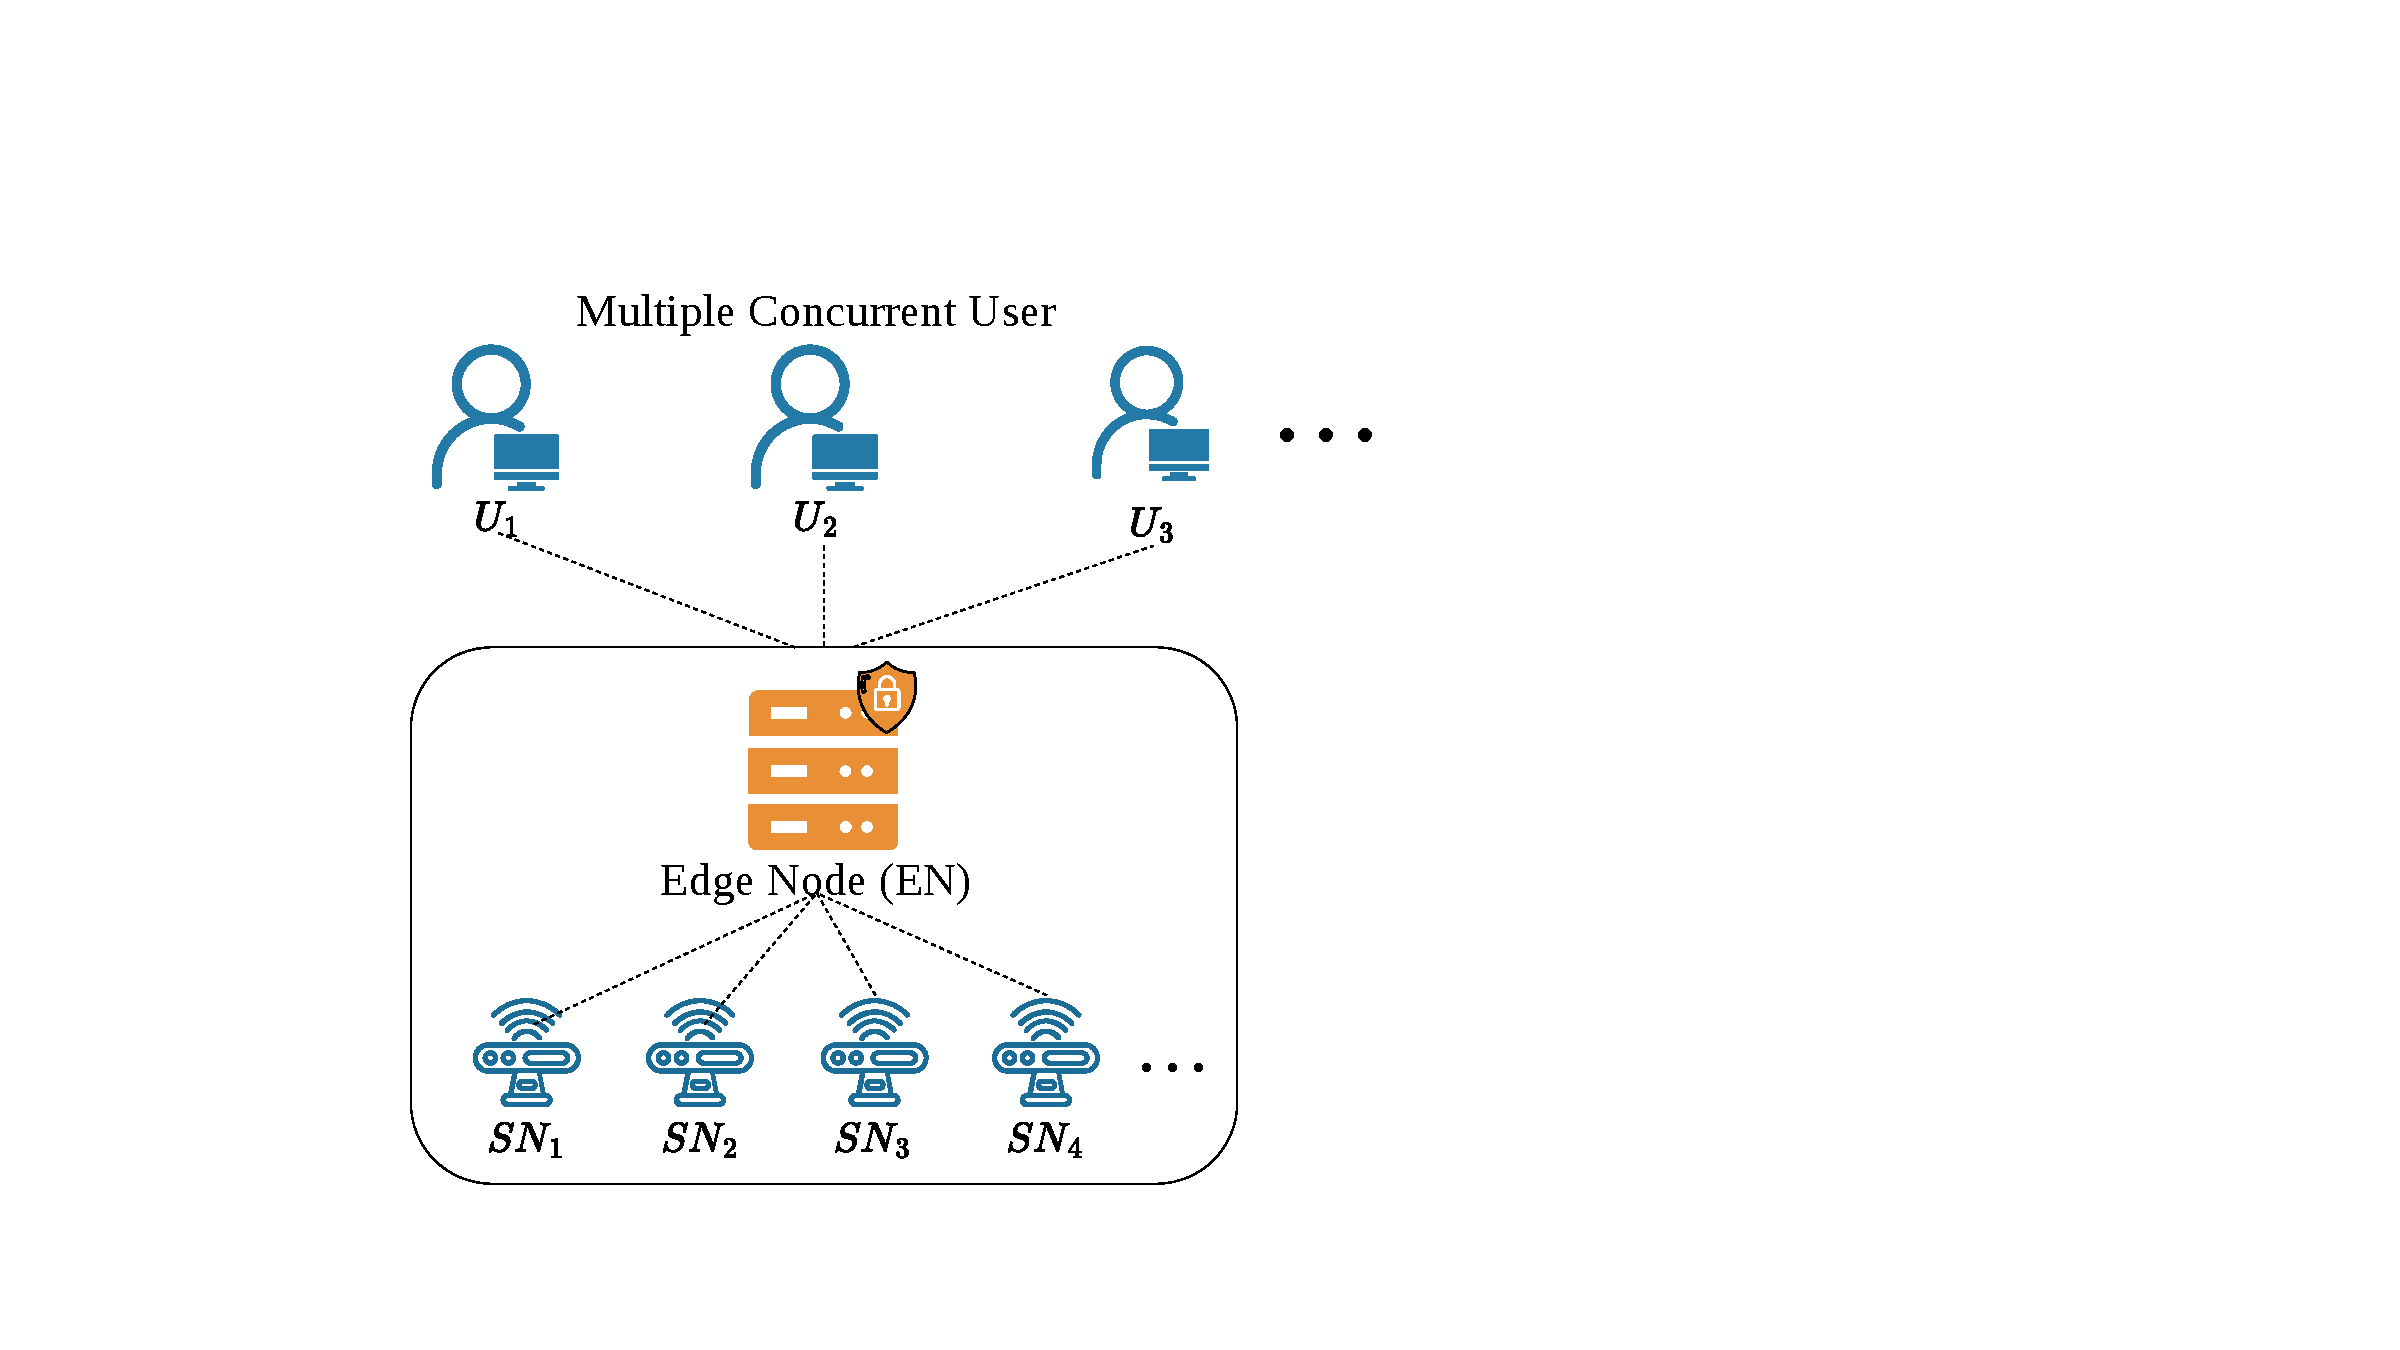
\includegraphics[width=0.4\textwidth]{netmodel.pdf}
\caption{Network model of the edge-collaborative IIoT scheme.}
\label{fig:netmodel}
\end{figure}

\subsection{The Edge Node as a Pre-Inference Control Point}\label{sec:guardrail}

Figure~\ref{fig:netmodel} is usually read as a routing diagram. Under edge intelligence it is better read as a control diagram, because two distinct paths converge on $EN$ and both of them terminate at the local model rather than at a data store.

On the request path, $U$ authenticates to $EN$ and, only after the four-credential transcript check succeeds, obtains a session in which it may issue a query against the sensing service and, in a deployment that hosts analytics, against the inference service exposed by the same node. An unauthorized request at this position is not merely an unauthorized read: it is an unauthorized query against a deployed model. Such access enables model extraction through repeated queries and membership inference against queried records \cite{tramer2016stealing,shokri2017membership}. On the ingestion path, $SN$ authenticates to $EN$ under $TC_j$ before its measurements are accepted into the aggregation that feeds local processing. An unauthorized sensor at this position is a channel through which fabricated observations reach the model's input, which is the deployment-time analogue of data poisoning \cite{nist2025aml,carlini2024poisoning}. The protocol is agnostic to what the local pipeline computes; what it fixes is the pair of admission decisions in front of it.

The assets guarded are therefore the model-query interface, the local inference service, and the sensor-input path, together with the session key that protects the resulting user--sensor exchange. Table~\ref{tab:coverage} states which attacks against those assets this paper claims to address and which it deliberately leaves to the model-level layer, so that the security claims of Sections~\ref{sec:security} and~\ref{sec:eval} are read against a fixed boundary.

\begin{table}[t]
\caption{Coverage of the authentication guardrail at an AI-enabled edge node.}
\label{tab:coverage}
\begin{tabularx}{\textwidth}{Xcl}
\toprule
\textbf{Attack or exposure} & \textbf{Addressed here} & \textbf{Where}\\
\midrule
Unauthenticated access to the model-query or inference interface & Y & Sec.~\ref{sec:aka}, $Q_1$\\
Unauthenticated or spoofed sensor input entering the aggregation path & Y & Secs.~\ref{sec:registration},~\ref{sec:aka}\\
Offline attack using a leaked verifier or recorded transcript & Partly & Secs.~\ref{sec:ceafsec},~\ref{sec:ror}\\
Exposure of up to three of the four credentials & Partly$^{a}$ & Sec.~\ref{sec:ror}\\
Replay, modification, impersonation, man-in-the-middle & Y & Sec.~\ref{sec:security}\\
Endpoint identity exposure to a channel observer & Y$^{b}$ & Sec.~\ref{sec:security}\\
Loss of one authentication message (credential desynchronization) & Y$^{c}$ & Sec.~\ref{sec:desync}\\
Distributed flooding of the edge node & Partly$^{d}$ & Sec.~\ref{sec:security}\\
\midrule
Prompt injection against a generative component & N & Sec.~\ref{sec:aisec}\\
Training-data or model poisoning after admission & N & Sec.~\ref{sec:aisec}\\
Adversarial examples at inference time & N & Sec.~\ref{sec:aisec}\\
Extraction or membership inference by an authenticated client & N$^{e}$ & Sec.~\ref{sec:aisec}\\
Detection of AI-assisted malware, ransomware, or intrusion & N & outside scope\\
Extraction of TEE-protected edge secrets & N & Sec.~\ref{sec:netmodel}\\
\bottomrule
\end{tabularx}
\noindent{\footnotesize $^{a}$ With $(SC,PW,BIO)$ exposed, a recorded $Q_1$ permits offline enumeration of the CEAF response; live attempts remain subject to deployment source/global limits, but no offline resistance is claimed. $^{b}$ Anonymity from the channel, not from $EN$. $^{c}$ The two-record window absorbs one lost $M_1$--$M_4$ message; repeated sensor-side loss invokes authenticated $M_{R1}$--$M_{R2}$ recovery, while credential update uses a separate bounded authenticated retry. $^{d}$ Source/global ingress and concurrency limits reduce processing pressure but do not prevent distributed flooding. $^{e}$ The guardrail bounds \emph{who} may query, which reduces the population able to mount such attacks, but gives no protection once a client is authenticated.}
\end{table}

\subsection{Threat Model}\label{sec:threat}

We use the Dolev--Yao model \cite{liu2019robust,liu2021sgx,li2019twofactor}. The adversary $\advA$ may:

\begin{itemize}
\item control both public channels by eavesdropping, replaying, modifying, dropping, and injecting protocol messages, and also act as a registered malicious user;
\item compromise at most two of the password, smart card, biometric, and CEAF credentials in the general model; we additionally analyze simultaneous exposure of the password, smart card, and biometric, in which case a recorded $Q_1$ permits offline CEAF enumeration and live attempts remain rate controlled. The latter is a deliberately separate stress test: it diagnoses the residual CEAF entropy after three-credential exposure and does not replace the general two-corruption ROR experiment;
\item capture a sensor and read all of its storage; security then concerns lateral compromise of uncaptured nodes, while the captured node itself requires revocation or re-registration;
\item access edge hardware but not extract TEE-protected secrets; and
\item observe the displayed challenge and selected CEAF response for at most one successful login. This observation does not by itself expose the password, card state, or biometric; combining it with all three is full credential compromise and is outside the security claim. Two consecutive CEAF observations recover $(\mathbf{N},\mathbf{N}_S)$ and are likewise excluded; this is an environmental observation bound, not a cryptographic guarantee; and
\item automate password guessing or biometric synthesis. Automation changes the rate and per-attempt success probability, not the set of values obtainable by $\advA$. Offline work against a password verifier or biometric template is assumed to proceed at the adversary's hardware speed. The one-successful-login limit on CEAF observation is a modeling assumption and is revisited in Section~\ref{sec:conclusions}.
\end{itemize}

The adversary is correspondingly \emph{not} assumed to attack the model behind the guardrail. Adversarial examples, poisoning of the locally hosted model, prompt injection against a generative component, and extraction or membership inference mounted from a session that has already been admitted are excluded by assumption rather than defended against; Table~\ref{tab:coverage} records the division and Section~\ref{sec:aisec} identifies the layer to which those attacks belong. A registered malicious user may deviate arbitrarily in the protocol, but no claim is made about what it does with the inference service once a session is established.

Corruption of $R_i$, $TC_i$, $TC_j$, or $R_{EN}$ makes a main-protocol session non-fresh because these values reconstruct transcript nonces. Hash inversion, second-preimage construction, collision finding, nonce prediction, and compromise of the secure registration channel are assumed infeasible. All claims in Section~\ref{sec:security} are scoped to these freshness and compromise conditions.

\subsection{Notation}

The notation used throughout this paper is listed in Table~\ref{tab:notation}.

\begin{table}[t]
\caption{Notation definitions.}
\label{tab:notation}
\begin{tabularx}{\textwidth}{lX}
\toprule
\textbf{Symbol} & \textbf{Meaning}\\
\midrule
$U,\ EN,\ SN$ & User, edge node, sensor node\\
$LD,\ SC$ & User device and smart card\\
$SA,\ \advA$ & System administrator, adversary\\
$ID_i, ID_{SC}, ID_{SN}, ID_{EN}$ & Unique identities of $U$, $SC$, $SN$, $EN$\\
$PID_i, PID_j$ & Persistent pseudo-identities of $U$ and $SN$\\
$PID_{SN}$ & One-time pseudo-identity of $SN$\\
$PW_i,\ SK$ & User static password and session key\\
$TS,\ \Delta T,\ \sigma$ & Timestamp, acceptance window, and $160$-bit challenge seed\\
$r_R,\ C_R^{cur},\ C_R^{prev}$ & Resynchronization nonce and masked sensor-version identifiers\\
$RS,\ \mathsf{Exp}(\cdot)$ & Challenge $RS=\mathsf{Exp}(\sigma)\in\Sigma^{L}$ and its expansion function\\
$s,\ \ell,\ L$ & Segment count, segment length, challenge length $L=s\ell$\\
$\mathbf{N},\ \mathbf{N}_S$ & CEAF offset vector and step vector in $\mathbb{Z}_{26}^{s}$\\
$DPW$ & One-time CEAF response $\CT_{\mathbf{N}}(RS)$\\
$\Gen(\cdot)/\Rep(\cdot)$ & Generation/reproduction algorithm of the fuzzy extractor\\
$\CT_{\mathbf{N}}(\cdot)$ & Segmented cognitive-binding primitive with offset vector $\mathbf{N}$\\
$h(\cdot),\ \cc,\ \oplus$ & Hash function, concatenation, XOR\\
$\operatorname{enc}_s,\operatorname{dec}_s$ & Fixed-length encoding of $\mathbb{Z}_{26}^{s}$ and its inverse on the encoding image\\
$T_H,\ T_F$ & Analytical unit costs of one hash and one fuzzy-extractor operation; values are illustrative\\
\bottomrule
\end{tabularx}
\end{table}

%%%%%%%%%%%%%%%%%%%%%%%%%%%%%%%%%%%%%%%%%%
\section{The Proposed Scheme}\label{sec:scheme}

The scheme has initialization, registration, login, AKA, and update phases. Verification is divided between two locations: $LD$ checks the password, card, and biometric, while $EN$ checks CEAF through the first protocol authenticator. The transcript binding prevents a verifier from being stored on the card, but a recorded $Q_1$ can still be tested offline after the other three credentials are exposed. Apart from fuzzy reproduction and challenge expansion, the protocol uses hashes, XOR, nonces, and timestamps. Rotating pseudo-identities and CEAF state are maintained as version-bound two-record windows to tolerate one lost authentication message. Protocol displays are numbered $(P1),(P2),\ldots$ for implementation reference; the analytical security bounds use ordinary equation numbers (1)--(3).

\subsection{System Initialization Phase}

Before deployment, the system administrator $SA$ provisions each device as follows:

\begin{enumerate}
\item Install the primitive set $\{\oplus, h(\cdot), \cc\}$ on every $LD$, $EN$, and $SN$.
\item Install $\mathsf{Exp}(\cdot)$ from Section~\ref{sec:challenge} on every $LD$ and $EN$; install $\CT_{\mathbf{N}}(\cdot)$ on every $EN$ and in the $LD$ display routine, and install $\{\Gen(\cdot),\Rep(\cdot)\}$ on every $LD$.
\item Fix the CEAF parameters $(s,\ell)$ and timestamp-acceptance window $\Delta T$ system-wide; this paper uses $(3,7)$. Let $\langle\cdot\rangle=\operatorname{enc}_s(\cdot)$ denote the fixed-length $160$-bit encoding of a vector in $\mathbb{Z}_{26}^{s}$, and let $\operatorname{dec}_s$ be its inverse on the encoding image. Thus $\operatorname{dec}_s$ is string decoding, not group inversion. Source/global ingress budgets are deployment parameters and are not stored in $\Lambda_i$.
\item Assign a unique identity $ID_{SC}$ to each smart card, $ID_{SN}$ to each sensor node, and $ID_{EN}$ to the edge node. Each edge domain samples one master secret $R_{EN}$ and seals it inside the TEE before any registration.
\end{enumerate}

\subsection{Registration Phase}\label{sec:registration}

Registration uses a secure channel and binds each user to a unique smart card and each sensor to the edge domain. Long-term credentials are stored in masked form, and $R_{EN}$ remains inside the TEE. The user sends the CEAF vectors to $EN$ only during registration and erases the working copies on $LD$; this placement prevents the card or login device from becoming a CEAF verification oracle.

\subsubsection{User Registration}

\begin{enumerate}
\item $U$ supplies its identity, password, biometric, and CEAF vectors. $LD$ reads $ID_{SC}$, samples $R_i$, obtains $TS_1$, and computes

\begin{ceq}
\begin{adjustbox}{max width=\columnwidth}
$\displaystyle\begin{aligned}
(R_U, P_U) &= \Gen(BIO_i),\\
UID_i &= h(ID_i \cc PW_i),\\
HPW &= h(ID_i \cc PW_i \cc ID_{SC} \cc R_U \cc R_i),
\end{aligned}$
\end{adjustbox}
\end{ceq}

then sends the registration tuple
\begin{ceq}
\begin{adjustbox}{max width=\linewidth}
$\{UID_i, ID_{SC}, HPW, R_i, \langle\mathbf{N}\rangle, \langle\mathbf{N}_S\rangle, TS_1\}$
\end{adjustbox}
\end{ceq}
to $EN$ over the secure channel and erases the CEAF vectors.

\item After checking $TS_1$, $EN$ uses its TEE-resident domain secret $R_{EN}$, obtains $TS_2$, and computes

\begin{ceq}
\begin{adjustbox}{max width=\columnwidth}
$\displaystyle\begin{aligned}
TC_i &= h(R_{EN} \cc R_i),\\
PID_i &= h(UID_i \cc ID_{SC} \cc R_i),\\
PTC_i &= TC_i \oplus h(R_i \cc UID_i \cc HPW),\\
RPW &= h(TC_i \cc R_i),
\end{aligned}$
\end{adjustbox}
\end{ceq}

returns $\{PID_i, RPW, PTC_i, TS_2\}$ to $LD$. $EN$ then forms the masked credential state

\begin{ceq}
\begin{adjustbox}{max width=\columnwidth}
$\displaystyle\begin{aligned}
PK_i &= R_i \oplus h(R_{EN} \cc ID_{EN}),\\
PN_{EN} &= \langle\mathbf{N}\rangle \oplus h(TC_i \cc R_{EN}),\\
PNS_{EN} &= \langle\mathbf{N}_S\rangle \oplus h(TC_i \cc ID_{EN} \cc R_{EN}),
\end{aligned}$
\end{adjustbox}
\end{ceq}

and stores the two-record state
\begin{ceq}
\begin{adjustbox}{max width=\linewidth}
$\displaystyle\Lambda_i=\{PID_i^{cur},PID_i^{prev},PK_i,PN_{EN},PNS_{EN}\},$
\end{adjustbox}
\end{ceq}
with $PID_i^{cur}=PID_i^{prev}=PID_i$. Because $PK_i$ is masked by $R_{EN}$ rather than $PID_i$, only the rotating identifier is duplicated. The CEAF vectors remain only at $EN$; invalid authentication attempts do not modify this record.

\item After checking $TS_2$, $LD$ computes
\begin{ceq}
$\displaystyle PR_i = R_i \oplus h(UID_i \cc ID_{SC} \cc R_U)$
\end{ceq}
and stores the five fields $PID_i$, $RPW$, $PTC_i$, $PR_i$, and $P_U$, then erases its working secrets. The provisioned public identifier $ID_{SC}$ is not counted as cryptographic state, and $SC$ stores no CEAF representation.
\end{enumerate}

\subsubsection{Sensor-Node Registration}

Sensor registration proceeds as follows.

\begin{enumerate}
\item $SN$ takes its own identity $ID_{SN}$, samples $R_j$, computes $PID_j=h(ID_{SN}\cc R_j)$ and $TC_j=h(R_j\cc ID_{SN}\cc ID_{EN})$, obtains $TS_1$, and sends $\{ID_{SN}, R_j, TS_1\}$ to $EN$. It retains $PID_j$ until the returned state is installed.
\item Upon receipt, $EN$ first checks the freshness of $TS_1$; if it has expired, $EN$ aborts. Otherwise $EN$ obtains $TS_2$ and computes

\begin{ceq}
\begin{adjustbox}{max width=\columnwidth}
$\displaystyle\begin{aligned}
PID_j &= h(ID_{SN} \cc R_j),\\
TC_j &= h(R_j \cc ID_{SN} \cc ID_{EN}),\\
PK_j &= R_j \oplus h(PID_j \cc ID_{EN}),\\
PTC_j &= TC_j \oplus PID_j,
\end{aligned}$
\end{adjustbox}
\end{ceq}

returns $\{PTC_j, TS_2\}$ to $SN$, and stores the two-record state $\Lambda_j=\{PID_j^{cur}, PID_j^{prev}, PK_j\}$ indexed by $ID_{SN}$, with $PID_j^{cur}=PID_j^{prev}=PID_j$.

\item Upon receipt, $SN$ first checks the freshness of $TS_2$; if it has expired, $SN$ aborts. Otherwise $SN$ stores $\{PID_j^{cur},PID_j^{prev},PTC_j^{cur},PTC_j^{prev}\}$, with both $PID$ entries initialized to $PID_j$ and both $PTC$ entries initialized to $PTC_j$; it then erases $R_j$ and $TC_j$.
\end{enumerate}

\subsection{User Login Phase}\label{sec:login}

The login phase separates local screening from remote authentication. $LD$ first rejects an incorrect password, card, or biometric without creating network traffic. It then collects only the CEAF response; $EN$ verifies that response through $M_1$. This order limits unnecessary edge and sensor work while preserving the requirement that the fourth credential be checked against edge-only state.

\textbf{(1) Verification of the first three credentials (static password, smart card, biometric).} $U$ inserts $SC$ into $LD$, inputs $\{ID_i, PW_i\}$, and provides biometric $BIO_i$. $LD$ reads the smart-card state and computes

\begin{ceq}
\begin{adjustbox}{max width=\columnwidth}
$\displaystyle\begin{aligned}
UID_i &= h(ID_i \cc PW_i),\\
R_U &= \Rep(P_U, BIO_i),\\
R_i &= PR_i \oplus h(UID_i \cc ID_{SC} \cc R_U),\\
HPW &= h(ID_i \cc PW_i \cc ID_{SC} \cc R_U \cc R_i),\\
TC_i &= PTC_i \oplus h(R_i \cc UID_i \cc HPW),\\
RPW^{*} &= h(TC_i \cc R_i).
\end{aligned}$
\end{adjustbox}
\end{ceq}

If $RPW^{*}\neq RPW$, $LD$ rejects; otherwise the first three credentials pass.

\textbf{(2) CEAF collection.} $U$ selects the target sensor $ID_{SN}$ and verifies the target shown by $LD$. $LD$ then samples $\sigma$, displays the candidate columns for $RS=\mathsf{Exp}(\sigma)$, and receives $DPW$. It retains $(\sigma,RS,DPW)$ only through $M_1$ construction and does not verify $DPW$. $U$ advances the offset only after session confirmation.

\subsection{Authentication and Key Agreement Phase}\label{sec:aka}

$U$, $EN$, and $SN$ authenticate, establish $SK$ for $U$ and $SN$, and rotate credentials. $M_1$ binds the four-credential login and target sensor, $M_2$ carries the edge contribution to the selected sensor, $M_3$ returns the sensor contribution, and $M_4$ confirms both nonces to the user. Because $EN$ is trusted, it learns $X$, $Y$, and therefore $SK$ (A15); it verifies the CEAF in step~(2). The timestamps provide freshness, whereas the $Q$ values bind the reconstructed fields and prevent an adversary from changing a timestamp or masked nonce independently.

All replay and concurrency checks are atomic. Within $\Delta T$, $EN$ caches $(PID_i,Q_1,TS_1)$ for $M_1$, and $SN$ caches $(PID_j,Q_2,TS_2)$ for $M_2$. For $M_3$ and $M_4$, $EN$ and $LD$ cache $(Q_3,TS_3)$ and $(Q_4,TS_4)$, respectively. A duplicate is rejected before any state transition. $LD$ retains one outstanding local context; $EN$ and $SN$ allow at most one accepted in-flight session for the relevant user and sensor records. $M_3$ must match the sole pending sensor context at $EN$, and $M_4$ must match the outstanding context at $LD$. Reservations and replay entries expire after $\Delta T$. These bounded caches and locks are required protocol metadata but are excluded from the static cryptographic-storage comparison in Section~\ref{sec:eval}.

\textbf{(1)} $LD$ samples a fresh random number $X$, obtains a timestamp $TS_1$, and computes

\begin{ceq}
\begin{adjustbox}{max width=\columnwidth}
$\displaystyle\begin{aligned}
PKS_1 &= X \oplus h(R_i \cc TC_i \cc TS_1),\\
PRS &= \sigma \oplus h(X \cc TC_i \cc TS_1),\\
PID_{SN} &= ID_{SN} \oplus h(X \cc TC_i),\\
Q_1 &= h(X \cc ID_{SN} \cc PID_i \cc RS \cc DPW \cc TS_1).
\end{aligned}$
\end{adjustbox}
\end{ceq}

$LD$ sends
\begin{ceq}
$M_1=\{PID_i, PKS_1, PRS, PID_{SN}, Q_1, TS_1\}$
\end{ceq}
to $EN$ and erases $DPW$. $Q_1$ binds the untransmitted response, while $PRS$ masks the challenge seed.

\textbf{(2)} Upon receipt, $EN$ checks the freshness of $TS_1$ and the $M_1$ replay key; if either check fails, $EN$ aborts. Otherwise $EN$ first searches for a state $\Lambda_i$ whose $PID_i^{cur}$ equals the received $PID_i$ and records $v_i=cur$. If no current value matches, it searches the previous values and records $v_i=prev$. If neither value matches or the record already has an in-flight session, $EN$ aborts. Source/global ingress and concurrency controls are applied independently of $PID_i$; they may reject traffic before this step but never create a user-specific lock. $EN$ then recovers

\begin{ceq}
\begin{adjustbox}{max width=\linewidth}
$\displaystyle\begin{aligned}
R_i &= PK_i \oplus h(R_{EN} \cc ID_{EN}),\\
TC_i &= h(R_{EN} \cc R_i),\\
X &= PKS_1 \oplus h(R_i \cc TC_i \cc TS_1),\\
\sigma &= PRS \oplus h(X \cc TC_i \cc TS_1),\quad RS=\mathsf{Exp}(\sigma),\\
ID_{SN} &= PID_{SN} \oplus h(X \cc TC_i),\\
\mathbf{N} &= \operatorname{dec}_s\bigl(PN_{EN} \oplus h(TC_i \cc R_{EN})\bigr),\\
\mathbf{N}_S &= \operatorname{dec}_s\bigl(PNS_{EN} \oplus h(TC_i \cc ID_{EN} \cc R_{EN})\bigr),\\
Q_1^{*} &= h(X \cc ID_{SN} \cc PID_i \cc RS \cc \CT_{\mathbf{N}}(RS) \cc TS_1).
\end{aligned}$
\end{adjustbox}
\end{ceq}

If $Q_1$ fails and $v_i=prev$, $EN$ retries once with $\mathbf{N}^{-}=\mathbf{N}-\mathbf{N}_S\bmod26$; it never tries $\mathbf{N}^{-}$ for $PID_i^{cur}$. A match adopts the preceding offset. Any other mismatch aborts without changing $\Lambda_i$ or any user-specific availability state. After a valid $Q_1$, $EN$ atomically inserts the $M_1$ replay key and reserves the user record. Acceptance jointly verifies the four credentials. $EN$ then retrieves $\Lambda_j$; if its sensor record is busy, $EN$ releases the user reservation and aborts. Otherwise it reserves that record, uses $PID_j^{cur}$, obtains $TS_2$, and computes

\begin{ceq}
\begin{adjustbox}{max width=\columnwidth}
$\displaystyle\begin{aligned}
R_j &= PK_j \oplus h(PID_j \cc ID_{EN}),\\
TC_j &= h(R_j \cc ID_{SN} \cc ID_{EN}),\\
PKS_2 &= X \oplus h(TC_j \cc TS_2),\\
Q_2 &= h(X \cc PID_j \cc TS_2),
\end{aligned}$
\end{adjustbox}
\end{ceq}

and sends $M_2=\{PID_j, PKS_2, Q_2, TS_2\}$ to the $SN$ designated by $ID_{SN}$.

\textbf{(3)} After checking $TS_2$, the $M_2$ replay key, and the absence of another in-flight session, $SN$ first matches the received $PID_j$ against the stored current/previous pair. If neither identifier matches, it invokes the authenticated resynchronization of Section~\ref{sec:resync} and does not process $M_2$. Otherwise, with $v_j\in\{cur,prev\}$ denoting the matching version, $SN$ recovers $TC_j=PTC_j^{v_j}\oplus PID_j$ and $X$, then verifies $Q_2$. If the check fails, it aborts without changing state. On success it atomically inserts the replay key, reserves the record, obtains $TS_3$, samples $Y$, derives $SK=h(X\cc Y)$, and computes

\begin{ceq}
\begin{adjustbox}{max width=\columnwidth}
$\displaystyle\begin{aligned}
PKS_3 &= Y \oplus h(TC_j \cc X \cc TS_3),\\
Q_3 &= h(X \cc Y \cc TS_3),
\end{aligned}$
\end{adjustbox}
\end{ceq}

then sends
\begin{ceq}
$M_3=\{PKS_3,Q_3,TS_3\}$
\end{ceq}
and derives $PID_j^{*}=PID_j\oplus h(Y\cc TS_3)$ and $PTC_j^{*}=TC_j\oplus PID_j^{*}$. It atomically shifts the sensor state to $(PID_j^{*},PID_j,PTC_j^{*},PTC_j)$, then releases its reservation while retaining the replay entry for $\Delta T$.

\textbf{(4)} After checking $TS_3$, matching $M_3$ to the pending sensor context, and rejecting a cached $M_3$ key, $EN$ recovers $Y$ and verifies $Q_3$. It then atomically inserts the replay key, obtains $TS_4$, and computes

\begin{ceq}
\begin{adjustbox}{max width=\columnwidth}
$\displaystyle\begin{aligned}
PKS_4 &= Y \oplus h(R_i \cc TC_i \cc X \cc TS_4),\\
Q_4 &= h(X \cc Y \cc TS_4),
\end{aligned}$
\end{adjustbox}
\end{ceq}

and sends $M_4=\{PKS_4, Q_4, TS_4\}$ to the $LD$ held by $U$. $EN$ then advances both credential states, keeping the value it has just used as the previous entry:

\begin{ceq}
\begin{adjustbox}{max width=\columnwidth}
$\displaystyle\begin{aligned}
PID_j^{*} &= PID_j \oplus h(Y \cc TS_3),\quad PK_j^{*} = R_j \oplus h(PID_j^{*} \cc ID_{EN}),\\
PID_i^{*} &= PID_i \oplus h(X \cc TS_4),\quad \mathbf{N}^{*}=\mathbf{N}+\mathbf{N}_S \bmod 26,\\
PN_{EN}^{*} &= \langle\mathbf{N}^{*}\rangle \oplus h(TC_i \cc R_{EN}),
\end{aligned}$
\end{adjustbox}
\end{ceq}

\begin{ceq}
\begin{adjustbox}{max width=\columnwidth}
$\displaystyle\begin{aligned}
\{PID_j^{prev}, PID_j^{cur}, PK_j\} &\leftarrow \{PID_j, PID_j^{*}, PK_j^{*}\},\\
\{PID_i^{prev}, PID_i^{cur}, PN_{EN}\} &\leftarrow \{PID_i, PID_i^{*}, PN_{EN}^{*}\}.
\end{aligned}$
\end{adjustbox}
\end{ceq}

Here $PID_i$ and $PID_j$ are the values used in this round; $PK_i$ and $PNS_{EN}$ remain unchanged. After the atomic commit, $EN$ releases both in-flight reservations while retaining the replay entries until they expire.

\textbf{(5)} After checking $TS_4$, matching the sole outstanding context, and rejecting a cached $M_4$ key, $LD$ recovers $Y$, derives $SK$, and verifies $Q_4$. It then atomically caches the key, stores $PID_i^{*}=PID_i\oplus h(X\cc TS_4)$, consumes the outstanding context, and signals success, after which $U$ advances $\mathbf{N}$. If $M_4$ is lost, $U$ retains the old state and step~(2) absorbs the next login.

\subsubsection{Two-record state and the desynchronization invariant}\label{sec:desync}

$SN$ commits when it sends $M_3$, $EN$ when it sends $M_4$, and $U$ after verifying $M_4$. A single lost $M_3$ or $M_4$ therefore leaves adjacent principals at most one round apart, which the two-record window absorbs. If repeated loss moves $SN$ beyond the identifiers retained by $EN$, the normal exchange stops and the authenticated recovery below is invoked; no unauthenticated rollback is allowed. The invariant protects state consistency, not availability under sustained loss: recovery still depends on delivery of the authenticated resynchronization exchange.

Each rotating value is therefore held as a version-bound $(cur,prev)$ pair:

\begin{ceq}
\begin{adjustbox}{max width=\columnwidth}
$\displaystyle\begin{aligned}
EN&: (PID_i^{cur},\mathbf{N}),\ (PID_i^{prev},\mathbf{N}-\mathbf{N}_S),\ (PID_j^{cur},PID_j^{prev}),\\
SN&: (PID_j^{cur},PID_j^{prev},PTC_j^{cur},PTC_j^{prev}).
\end{aligned}$
\end{adjustbox}
\end{ceq}

$\mathbf{N}^{-}$ is recomputed from $(\mathbf{N},\mathbf{N}_S)$, avoiding another stored copy. A current $PID_i$ is verified only with $\mathbf{N}$, whereas $\mathbf{N}^{-}$ is available only after a previous-$PID_i$ match. Thus identifiers and CEAF offsets cannot be mixed across versions: a current identifier is never tested with the previous offset, and a previous identifier is never promoted to the current version without the adjacent-state commit. A previous-value match is accepted only for the immediately adjacent state and is followed by the normal commit rule. Together with the replay cache and single-session reservation, this one-round window recovers one lost $M_1$--$M_4$ without accepting a duplicate transcript. Repeated sensor-side loss is handled only by the authenticated resynchronization below; credential update remains separate.

\subsubsection{Authenticated sensor resynchronization}\label{sec:resync}
\begingroup\small

If $SN$ receives an $M_2$ whose $PID_j$ matches neither stored identifier, it derives $TC_j=PTC_j^{cur}\oplus PID_j^{cur}$, samples fresh $(r_R,TS_R)$, and computes

\begin{ceq}
\begin{adjustbox}{max width=\columnwidth}
$\displaystyle\begin{aligned}
C_R^{cur} &= PID_j^{cur}\oplus h(TC_j\cc r_R\cc1),\\
C_R^{prev} &= PID_j^{prev}\oplus h(TC_j\cc r_R\cc2),\\
Q_R^{(1)} &= h(TC_j\cc C_R^{cur}\cc C_R^{prev}\cc r_R\cc TS_R\cc\mathrm{r1}),
\end{aligned}$
\end{adjustbox}
\end{ceq}

It sends $M_{R1}=\{C_R^{cur},C_R^{prev},r_R,Q_R^{(1)},TS_R\}$ and waits without changing state. $EN$ recovers $R_j$ from $(PID_j^{cur},PK_j)$, derives $TC_j$, checks freshness, replay, and $Q_R^{(1)}$, then cancels the stale $M_2$ context and releases its reservations. It recomputes $PK_j^{*}=R_j\oplus h(C_R^{cur}\cc ID_{EN})$, installs $(PID_j^{prev},PID_j^{cur},PK_j)=(C_R^{prev},C_R^{cur},PK_j^{*})$, and returns

\begin{ceq}
\begin{adjustbox}{max width=\columnwidth}
$\displaystyle Q_R^{(2)}=h(TC_j\cc C_R^{cur}\cc C_R^{prev}\cc r_R\cc TS_R\cc\mathrm{r2}),\qquad
M_{R2}=\{r_R,Q_R^{(2)},TS_R\}.$
\end{adjustbox}
\end{ceq}

$SN$ accepts $M_{R2}$ only for its outstanding $r_R$ and a valid $Q_R^{(2)}$. It then installs the four recovered fields
$(C_R^{cur},C_R^{prev},TC_j\oplus C_R^{cur},TC_j\oplus C_R^{prev})$ and clears the request. If the acknowledgement is lost, it retransmits the same $M_{R1}$ within $\Delta T$ and $EN$ returns the cached acknowledgement without another state transition. This idempotent exchange repairs repeated sensor-side loss when the two endpoints can still exchange authenticated messages; it is excluded from the normal-session cost and does not claim availability against distributed flooding or a permanently partitioned link.

\endgroup

\subsection{Credential Update Phase}\label{sec:update}

Password and biometric updates are card-local because they only change the masks used to recover $R_i$ and $TC_i$. Changing the edge-held CEAF vectors requires the protected exchange below. The update is executed only after a complete AKA run so that $LD$ and $EN$ can protect the new vectors with a fresh update key rather than with the user's low-entropy credentials.
The replay-cache and single-pending-context rules of Section~\ref{sec:aka} also apply to $M_5$ and $M_6$ within $\Delta T$. The update replay keys are $(Q_5,TS_5)$ at $EN$ and $(Q_6,TS_6)$ at $LD$. $LD$ keeps the pending update until a valid $M_6$ is received and retransmits the same $M_5$ after a timeout; $EN$ caches the accepted update and its $M_6$ for this retry window and resends it without a second state transition. Thus, one lost $M_6$ is recovered by an authenticated retry rather than by re-registration.

\begin{enumerate}
\item $LD$ completes Sections~\ref{sec:login}--\ref{sec:aka}; $U$ and $EN$ set $SK_{UE}=h(TC_i\cc X\cc Y)$.

\item $U$ selects any subset of a new password, biometric, CEAF vector, and CEAF step vector. An unchanged starred value equals its current value. For a password-only update, $(R_U^{*},P_U^{*})=(R_U,P_U)$; for a biometric-only update, $PW_i^{*}=PW_i$. If only one CEAF vector changes, the other starred vector equals its current value.

\item If the biometric changes, $LD$ obtains $(R_U^{*},P_U^{*})=\Gen(BIO_i^{*})$; otherwise it reuses $(R_U,P_U)$. It then recomputes the card-local values

\begin{ceq}
\begin{adjustbox}{max width=\linewidth}
$\displaystyle\begin{aligned}
UID_i^{*} &= h(ID_i \cc PW_i^{*}),\\
HPW^{*} &= h(ID_i \cc PW_i^{*} \cc ID_{SC} \cc R_U^{*} \cc R_i),\\
PTC_i^{*} &= TC_i \oplus h(R_i \cc UID_i^{*} \cc HPW^{*}),\\
PR_i^{*} &= R_i \oplus h(UID_i^{*} \cc ID_{SC} \cc R_U^{*}),
\end{aligned}$
\end{adjustbox}
\end{ceq}

If neither CEAF vector changes, $LD$ atomically commits the five card fields, using $PTC_i^{*}$, $PR_i^{*}$, and $P_U^{*}$, and erases the working values. The update then ends without contacting $EN$. If either CEAF vector changes, $LD$ obtains $TS_5$ and computes

\begin{ceq}
\begin{adjustbox}{max width=\columnwidth}
$\displaystyle\begin{aligned}
C_1 &= \langle\mathbf{N}^{*}\rangle \oplus h(SK_{UE} \cc 1 \cc TS_5),\\
C_2 &= \langle\mathbf{N}_S^{*}\rangle \oplus h(SK_{UE} \cc 2 \cc TS_5),\\
Q_5 &= h(SK_{UE} \cc \langle\mathbf{N}^{*}\rangle \cc \langle\mathbf{N}_S^{*}\rangle \cc TS_5),
\end{aligned}$
\end{adjustbox}
\end{ceq}

sending $M_5=\{C_1, C_2, Q_5, TS_5\}$ to $EN$.

\item Upon receiving $M_5$, $EN$ first checks its pending-update cache. If $(Q_5,TS_5)$ matches an accepted update still within the retry window, it retransmits the cached $M_6$ and makes no state change. Otherwise, after checking $TS_5$ and the replay key, $EN$ recovers
\begin{ceq}
\begin{adjustbox}{max width=\columnwidth}
$\displaystyle\begin{aligned}
\langle\mathbf{N}^{*}\rangle &= C_1 \oplus h(SK_{UE} \cc 1 \cc TS_5),\\
\langle\mathbf{N}_S^{*}\rangle &= C_2 \oplus h(SK_{UE} \cc 2 \cc TS_5).
\end{aligned}$
\end{adjustbox}
\end{ceq}
It verifies $Q_5$, obtains $TS_6$, and computes
\begin{ceq}
\begin{adjustbox}{max width=\columnwidth}
$\displaystyle\begin{aligned}
PN_{EN}^{*} &= \langle\mathbf{N}^{*}\rangle \oplus h(TC_i \cc R_{EN}),\\
PNS_{EN}^{*} &= \langle\mathbf{N}_S^{*}\rangle \oplus h(TC_i \cc ID_{EN} \cc R_{EN}),\\
Q_6 &= h(SK_{UE}\cc\langle\mathbf{N}^{*}\rangle\cc\langle\mathbf{N}_S^{*}\rangle\cc TS_6).
\end{aligned}$
\end{adjustbox}
\end{ceq}
$EN$ atomically stores the two starred masks, caches the accepted update and $M_6$, and returns $M_6=\{Q_6,TS_6\}$. It never applies an accepted update twice, and no failed $M_1$ attempt can alter this update state.

\item After checking $TS_6$ and verifying $M_6$ against both starred CEAF vectors, $LD$ commits any new card values and $U$ memorizes the new CEAF pair. Until this check succeeds, the old local values are retained. If $M_6$ is lost, $LD$ retransmits the unchanged $M_5$ within $\Delta T$; the cached response above is returned and the update is committed only once. If all retries expire, $LD$ reports an incomplete update and retains its old local values; loss-atomicity is not claimed outside this bounded retry window.
\end{enumerate}

%%%%%%%%%%%%%%%%%%%%%%%%%%%%%%%%%%%%%%%%%%
\subsection{Implementation-Oriented Message Summary}
The main exchange can be implemented from the following compact summary; a failed verification leaves the corresponding state unchanged. $M_1$ ($LD\rightarrow EN$) binds the four credentials, challenge, target sensor, and nonce in $Q_1$; $EN$ verifies CEAF and reserves the user record. $M_2$ ($EN\rightarrow SN$) carries the masked edge contribution and $Q_2$; $SN$ verifies the sensor context and derives its session contribution. $M_3$ ($SN\rightarrow EN$) returns the sensor contribution and $Q_3$; $SN$ shifts its two-record state after sending, while $EN$ verifies the pending context. $M_4$ ($EN\rightarrow LD$) confirms both nonces with $Q_4$; $LD$ verifies the session and commits its local identifier, while $EN$ commits the adjacent records. Optional $M_5$ ($LD\rightarrow EN$) and $M_6$ ($EN\rightarrow LD$) update the CEAF vectors under $SK_{UE}$; the cached $M_6$ recovers one lost update acknowledgement without a second state transition.

\section{Security Analysis}\label{sec:security}

The Real-or-Random (ROR) reduction bounds transcript and credential-guessing attacks, and the informal audit connects those results to Table~\ref{tab:security}. The claims are conditioned on the threat model and freshness rules of Section~\ref{sec:threat}; in particular, the main protocol claims neither PFS nor key opacity from $EN$.

\subsection{Formal Security Analysis}\label{sec:formal}

\subsubsection{Reduction in the Real-or-Random Model}\label{sec:ror}

Protocol instances answer $\mathsf{Execute}$, $\mathsf{Send}$, $\mathsf{Reveal}$, $\mathsf{Hash}$, $\mathsf{CorruptSC}$, $\mathsf{CorruptPW}$, $\mathsf{CorruptBIO}$, and $\mathsf{CorruptCEAF}$ queries, followed by one $\mathsf{Test}$ on a fresh accepted instance. $\mathsf{Execute}$ exposes honest transcripts, $\mathsf{Send}$ models active delivery and modification, and $\mathsf{Reveal}$ returns an accepted session key. The general experiment permits at most two credential corruptions for one user and represents the protocol's ordinary partial-compromise claim. A separate three-credential experiment exposes $(SC,PW,BIO)$ together but not the CEAF state; because $Q_1$ is public in a recorded transcript, the experiment includes offline enumeration of the $26^s$ possible responses, while live impersonation attempts remain subject to the edge verifier. This stress test is intentionally separated because it measures the residual CEAF entropy after the other credentials are lost; it complements, rather than replaces, the general ROR experiment. Exposure of all four credentials, reveal of the tested key, or corruption of a nonce-recovery value makes the tested session non-fresh. With $h$ a random oracle, $\mathsf{Adv}^{\mathrm{ror}}_\Pi(\advA)=|2\Pr[\mathsf{Succ}]-1|$.

Let $q_h,q_s,q_n$ count hash queries, active sends, and sampled nonces, with lengths $l_h,l_n$. Let $q_e$ count offline CEAF tests against recorded transcripts and $q_c$ count live CEAF trials admitted by the deployment's source/global policy and reaching the CEAF verifier. Each offline or live CEAF test consumes at least one random-oracle query, so the disjoint total $q_{\mathrm{CEAF}}=q_e+q_c$ satisfies $q_{\mathrm{CEAF}}\le q_h$ and $q_c\le q_s$. Under Zipf parameters $(C_z,\alpha)$ \cite{wangzipf} and biometric min-entropy $l_b$, the remaining password and biometric guessing probability satisfies Eq.~\eqref{eq:pcred}:
\begin{equation}
p_{\mathrm{cred}}(q_g)\le
 \min\left\{1,\ C_z\sum_{r=1}^{q_g}r^{-\alpha}+\frac{q_g}{2^{l_b}}\right\}
\label{eq:pcred}
\end{equation}
where $q_g$ counts password and biometric guesses, and $C_z r^{-\alpha}$ is the Zipf probability assigned to rank $r$. The deployment's source/global admission policy bounds $q_c$ per observation interval; this bound is not a per-user lock and is not assumed to hold for the entire credential lifetime.

The reduction begins with the real attack game $G_0$. Game $G_1$ aborts on any hash-output or nonce collision; the birthday terms below bound the statistical difference from $G_0$. Game $G_2$ additionally aborts when an active send contains a valid authenticator whose corresponding random-oracle input was never queried. Such an event is a direct tag forgery, bounded by the hash length and number of active sends. A previously accepted authenticator is instead rejected by the replay cache and cannot create a new accepted instance. In $G_3$, the test key is replaced by an independent random value unless the adversary queried $h(X\cc Y)$ for the tested session.

Producing that final query requires reconstructing the long-term masking path, testing CEAF responses against a recorded $Q_1$, obtaining an accepted live response, or forging a preceding authenticator. Password and biometric uncertainty is collected in $p_{\mathrm{cred}}$; the union of offline and live CEAF tests contributes $q_{\mathrm{CEAF}}/26^s$, with the live component bounded only by the deployment's source/global admission policy. Define $\varepsilon_{\mathrm{cred}}=\min\{1,2p_{\mathrm{cred}}(q_g)\}$ and $\varepsilon_{\mathrm{CEAF}}=\min\{1,2q_{\mathrm{CEAF}}/26^s\}$. Applying the triangle inequality across the games gives the ROR bound in Eq.~\eqref{eq:ror-bound}:
\begin{equation}
\begin{adjustbox}{max width=\columnwidth}
$\displaystyle
 \mathsf{Adv}^{\mathrm{ror}}_\Pi(\advA)
 \le \min\left\{1,\,
 \frac{q_h(q_h-1)}{2^{l_h}}
+ \frac{q_n(q_n-1)}{2^{l_n}}
+ \frac{2q_s}{2^{l_h}}
+ \varepsilon_{\mathrm{cred}}
 + \varepsilon_{\mathrm{CEAF}}\right\}.$
\end{adjustbox}
\label{eq:ror-bound}
\end{equation}

The bound makes two limits explicit. First, the CEAF contributes only $s\log_2 26=14.10$ bits at the selected parameters; a recorded transcript permits offline enumeration, while source/global admission control applies only to live attempts. Second, overall security depends on password distribution and biometric min-entropy rather than on the hash length alone. The outer minimum enforces the defining ROR range $\mathsf{Adv}\le1$; once $q_{\mathrm{CEAF}}\ge26^s/2$, the CEAF term saturates at the trivial bound rather than exceeding it. The main protocol excludes post-session long-term compromise.

In the three-credential experiment, $(SC,PW,BIO)$ are known and the tested CEAF state is not. For recorded transcripts, $q_e$ offline response tests replace the password/biometric term; live attempts additionally contribute $q_c$, with $q_e+q_c\le q_h$. The resulting three-credential bound is given in Eq.~\eqref{eq:three-cred-bound}:
\begin{equation}
\begin{adjustbox}{max width=\columnwidth}
$\displaystyle
 \mathsf{Adv}^{\mathrm{3cred}}_\Pi(\advA)
 \le \min\left\{1,\,
 \frac{q_h(q_h-1)}{2^{l_h}}
+ \frac{q_n(q_n-1)}{2^{l_n}}
+ \frac{2q_s}{2^{l_h}}
 + \varepsilon_{\mathrm{CEAF}}\right\}.$
\end{adjustbox}
\label{eq:three-cred-bound}
\end{equation}
This is a bounded enumeration-and-online-guessing statement, not a claim of offline resistance after exposure of the other three credentials.

To complement the symbolic ROR argument, a supplied HLPSL abstraction of the core $M_1$--$M_4$ exchange returned \texttt{SAFE} with both AVISPA OFMC and CL-AtSe under bounded sessions (OFMC: four visited nodes at depth three; CL-AtSe: eight analyzed and three reachable states, typed model). The abstraction targets message-level secrecy and authentication; offline CEAF enumeration, source/global rate control, two-record recovery, $M_5$--$M_6$ retry, TEE extraction, and human usability remain outside its scope.

\subsection{Protocol-Level Security Audit}\label{sec:informal}

\subsubsection{Resistance to First-Factor Recovery}

$Q_1$ binds the fresh challenge, CEAF response, target sensor, pseudo-identity, nonce, and timestamp. The card does not store a CEAF verifier, but a recorded $Q_1$ can be tested offline after the card, password, and biometric are exposed; live attempts are still checked at $EN$ and are subject only to deployment source/global admission limits. The response state advances only after confirmation, so a dropped attempt cannot move one side prematurely. As Section~\ref{sec:ceafsec} notes, two consecutive observations recover the CEAF state, and the protocol therefore makes no offline-resistance claim under three-credential compromise.

\subsubsection{Resistance to Sensor-Node Capture}

Capturing $SN_j$ reveals its stored masked credentials and, with an observed current $PID_j$, that node's $TC_j$; the adversary can then attack current or future sessions of the captured node until revocation, and the protocol claims no more. Because every sensor uses an independently sampled $R_j$ and a separate $TC_j$, this does not reconstruct another sensor's credential, so A4 concerns containment of lateral compromise to uncaptured nodes.

\subsubsection{Session-Key Independence and the Absence of Perfect Forward Secrecy}

Fresh independent $(X,Y)$ give session-key independence: before long-term compromise, keys from separate accepted sessions are independent even when transcripts are public. This is weaker than perfect forward secrecy. A recorded transcript together with later $(R_i,TC_i)$ or the edge record containing $R_{EN}$ and $PK_i$ recovers both nonces and past keys, so the main protocol lacks PFS; it protects $SK$ from a channel-only adversary, not from trusted $EN$. Thus A12 in Table~\ref{tab:security} must not be read as an A13 claim.

%%%%%%%%%%%%%%%%%%%%%%%%%%%%%%%%%%%%%%%%%%
\section{Comparison and Analytical Evaluation}\label{sec:eval}

We compare security properties with Li and Wang \cite{li2019twofactor}, Li et al. \cite{li2018ecc}, Far et al. \cite{far}, and Xu et al. \cite{xu}. Their three-tier architectures are sufficiently close for a qualified property comparison. Quantitative cross-protocol rankings are not reported because the papers use different operation sets, hardware platforms, point sizes, and storage-inclusion rules; reproducing them under one verified implementation is outside the present analytical study.

\subsection{Security-Property Comparison}

Table~\ref{tab:security} reports A12--A15 separately: key independence, PFS, update resilience, and edge-node key opacity.

Entries follow the original attack analyses and update procedures rather than a simple count of claimed features. A1 requires a cognitively evaluable factor that is verified remotely, not merely a dynamic identifier. A12 denotes independence of fresh session keys, whereas A13 requires resistance to later long-term compromise. A15 asks whether the authenticating intermediary can derive the endpoint key.

Far et al.'s PFS entry assumes erasure of its ephemeral value; its paper describes integrity checks and rollback after a token update, but not arbitrary-loss recovery, and its gateway derives the key. Xu et al. provide A13 and A15 under their ECC construction; their A14 concerns authority/control-node update consistency rather than packet-loss recovery. Our main protocol deliberately lacks A13 and A15. Its A2/A3 entries are qualified because a recorded $Q_1$ enables offline CEAF enumeration after three-credential exposure, while live attempts are subject to deployment source/global limits. Our A14 covers the normal $M_1$--$M_4$ exchange, authenticated sensor resynchronization, and the bounded authenticated retry of $M_5$--$M_6$; rate limiting does not justify marking A8 as full DDoS resistance.

Cui et al. \cite{cui} provide message authentication without a comparable session key; Shang et al. \cite{shang} use two parties without a user or smart card. They are therefore excluded from the three-party tables.

\begin{table}[t]
\caption{Security-property comparison.}
\label{tab:security}
\begin{tabularx}{\textwidth}{lYYYYY}
\toprule
\textbf{Property} & \textbf{Li and Wang \cite{li2019twofactor}} & \textbf{Li et al. \cite{li2018ecc}} & \textbf{Far et al. \cite{far}} & \textbf{Xu et al. \cite{xu}} & \textbf{Ours}\\
\midrule
A1  & N & N & N & N & Y\\
A2  & Y & Y & Y & Y & P$^{a}$\\
A3  & Y & Y & Y & Y & P$^{b}$\\
A4  & Y & Y & Y & Y & P$^{c}$\\
A5  & N & Y & Y & Y & Y\\
A6  & Y & Y & Y & Y & Y\\
A7  & Y & Y & Y & Y & Y\\
A8  & N & N & P$^{i}$ & P$^{i}$ & N\\
A9  & Y & Y & Y & Y & P$^{d}$\\
A10 & Y & Y & Y & Y & P$^{e}$\\
A11 & Y & Y & Y & Y & P$^{f}$\\
A12 & Y & Y & Y & Y & Y\\
\midrule
A13 & Y & Y & Y$^{g}$ & Y & N\\
A14 & Y & Y & P$^{j}$ & P$^{k}$ & P$^{h}$\\
A15 & Y & Y & N & Y & N\\
\bottomrule
\end{tabularx}

\noindent{\footnotesize Y denotes the property under the stated model; P denotes a partial or qualified property; N denotes that the property is not provided. A1: cognitively evaluable authentication credential verified remotely; A2: smart-card theft and offline guessing; A3: online guessing; A4: sensor capture; A5: three-factor authentication; A6: message integrity; A7: replay; A8: DDoS; A9: mutual authentication and impersonation; A10: anonymity; A11: tracking; A12: session-key independence; A13: PFS; A14: desynchronization; A15: opacity to the authenticating intermediary. $^{a}$ Card-only compromise requires joint guessing; card plus password or biometric permits offline guessing of the remaining credential. With $(SC,PW,BIO)$ exposed, a recorded $Q_1$ also permits offline CEAF enumeration. $^{b}$ A single admitted CEAF guess succeeds with probability $26^{-s}$; over $q_c$ admitted online trials, the union-bound success probability is at most $\min\{1,q_c/26^s\}$. The corresponding ROR advantage contribution is $2\min\{1,q_c/26^s\}$, while the full reduction also includes offline tests $q_e$. $^{c}$ The captured node remains compromised; P denotes containment of lateral compromise to other nodes. $^{d}$ Attribution at $U$ assumes an honest trusted relay. $^{e}$ Anonymity is from the public channel, not from $EN$. $^{f}$ P denotes passive unlinkability only; an active drop can link adjacent runs while the real identity remains hidden. $^{g}$ Follows the source paper's erasure assumption. $^{h}$ P covers $M_1$--$M_4$, authenticated sensor resynchronization, and the bounded authenticated $M_5$--$M_6$ retry, not arbitrary repeated loss. $^{i}$ Admission checks do not establish resistance to distributed flooding. $^{j}$ Integrity checks and token-update rollback address some state mismatches, not arbitrary loss. $^{k}$ Secure authority/control-node updates do not establish packet-loss recovery.}
\end{table}

\subsection{Analytical Overhead of the Proposed Scheme}

We report computation, communication, and storage for one complete login and AKA session; registration, update, replay caches, and session locks are excluded.

\subsubsection{Cost Model and Overhead}\label{sec:costmodel}

We neglect random generation, timestamps, XOR, display, and character shifts in the analytical count; challenge expansion has expected cost $2.000008T_H$, rounded to $2T_H$. Secrets, nonces, hashes, and identities are modeled as $160$ bits and timestamps as $32$ bits under the $H_{160}$ field profile defined in Section~\ref{sec:ceaf}. With illustrative unit costs $T_H=0.0004$\,ms and $T_F=0.442$\,ms, the main protocol is analytically estimated at $15T_H+T_F+21T_H+6T_H=42(0.0004)+0.442=0.4588$\,ms. This $0.4588$\,ms value is an illustrative analytical estimate, not an implementation benchmark. We additionally ran the reference implementation in \texttt{benchmarks/benchmark\_protocol.py} for 200,000 iterations on a Windows 10 host with an AMD Ryzen 7 7800X3D 8-core processor (16 logical CPUs), Python 3.14.2, and the OpenSSL-backed \texttt{hashlib} SHA-256 implementation. The median time of one full 64-byte SHA-256 operation was $T_H^{\mathrm{host}}=0.000425$\,ms (p95 $0.000454$\,ms); protocol-field truncation to 160 bits is applied after the hash operation. The reference 256-byte fuzzy reproduction was $T_F^{\mathrm{host}}=0.004376$\,ms (p95 $0.004569$\,ms). The resulting role medians were $0.011004$\,ms for $LD$ (15 hashes plus reproduction), $0.008994$\,ms for $EN$ (21 hashes), and $0.002625$\,ms for $SN$ (6 hashes), whose sum is $0.022624$\,ms. This is a host-software measurement, not a constrained-board, energy, or network benchmark; the fuzzy-reproduction value is implementation-dependent because the manuscript does not mandate a specific error-correcting fuzzy extractor. As an interim constrained-device calibration, Ledwaba et al. measured full SHA-256 on a Cortex-M4 at $57.361$\,$\mu$s/hash, $114.615$\,mW, and $3.56$\,kB of RAM \cite{ledwaba2018cortex}. The reported $114.615$\,mW is power, not per-hash energy; therefore, we first compute $E_H^{\mathrm{M4}}=P_H t_H=114.615\,\mathrm{mW}\times57.361\,\mu\mathrm{s}=6.574\,\mu\mathrm{J}=0.006574$\,mJ per hash, and then multiply by the role-specific hash counts. This gives the SHA-only estimates in Table~\ref{tab:overhead}, with the $LD$ fuzzy-reproduction time and energy left as $T_F$ and $E_F$. These are literature-calibrated estimates rather than measurements of this protocol; they exclude fuzzy extraction, I/O, radio, scheduling, compiler, and board-specific effects. Communication is $2048$ bits for a normal session and static state is $2880$ bits for $m=n=1$ under the 160-bit field profile; an edge domain with $m$ users and $n$ sensors stores $160+800m+640n$ bits at $EN$. The exceptional resynchronization exchange is excluded from the normal-session communication count. These counts exclude link, transport, retransmission, certificate, replay-cache, lock, and rate-limit overheads.

\begin{table}[t]
\caption{Analytical, host-measured, and literature-calibrated overhead of the proposed exchange. Communication and static-state entries use the 160-bit field profile; the $0.4588$\,ms value is an illustrative analytical estimate, host timing is a reference software measurement, and the Cortex-M4 row is a SHA-only estimate rather than a protocol benchmark.}
\label{tab:overhead}

\noindent\textbf{(a) Computation}\par\smallskip
\begin{tabularx}{\columnwidth}{lYYYcc}
\toprule
\textbf{Scheme} & \boldmath$U$ & \boldmath$EN$ & \boldmath$SN$ & \textbf{Analytical (ms)} & \textbf{Host median (ms)}\\
\midrule
Ours & $15T_H+T_F$ & $21T_H$ & $6T_H$ & 0.4588 & 0.0226\\
\bottomrule
\end{tabularx}

\smallskip\noindent\textbf{(b) Communication (bits)}\par\smallskip
\begin{tabularx}{\columnwidth}{llXY}
\toprule
\textbf{Msg} & \textbf{Route} & \textbf{Accounting} & \textbf{Main}\\
\midrule
$M_1$ & $LD\!\rightarrow\!EN$ & $5(160)+32$ & 832\\
$M_2$ & $EN\!\rightarrow\!SN$ & $3(160)+32$ & 512\\
$M_3$ & $SN\!\rightarrow\!EN$ & $2(160)+32$ & 352\\
$M_4$ & $EN\!\rightarrow\!LD$ & $2(160)+32$ & 352\\
\midrule
Total & & & 2048\\
\bottomrule
\end{tabularx}

\smallskip\noindent\textbf{(c) Static cryptographic state (bits)}\par\smallskip
\begin{tabularx}{\columnwidth}{lYYYc}
\toprule
\textbf{Scope} & \boldmath$SC/LD$ & \boldmath$EN$ & \boldmath$SN$ & \textbf{Total}\\
\midrule
Base case ($m=n=1$) & 800 & 1440 & 640 & 2880\\
\bottomrule
\end{tabularx}

\smallskip\noindent\textbf{(d) Literature-calibrated Cortex-M4 estimate (SHA-only)}\par\smallskip
\scriptsize
\begin{tabular}{lccc}
\toprule
\textbf{Role} & \textbf{SHA-256 calls} & \textbf{Time / energy (ms / mJ)} & \textbf{RAM reference}\\
\midrule
$LD$ & 15 & $0.860+T_F$ / $0.099+E_F$ & 3.56\,kB\\
$EN$ & 21 & $1.205$ / $0.138$ & 3.56\,kB\\
$SN$ & 6 & $0.344$ / $0.039$ & 3.56\,kB\\
\bottomrule
\end{tabular}\par\smallskip
\normalsize
\noindent{\footnotesize The estimates apply $E_H=P_Ht_H$ to the full-SHA-256 time and power reported for a Cortex-M4 in \cite{ledwaba2018cortex}; the reported power is not treated as an energy value, and $E_F$ is not estimated because the protocol leaves the fuzzy extractor implementation open.}
\end{table}

\subsection{Sensitivity of the Guardrail Parameters}\label{sec:sensitivity}

Because the live attack surface is the online CEAF term, the deployment parameters that shape that term are reported explicitly. The two protocol-relevant quantities are the segment count $s$, which fixes the response space $26^{s}$, and the admitted online attempt budget $q_{c}$ of Section~\ref{sec:ror}. The values below are computed from the expressions already derived and are not measurements; they describe the security budget, not an implementation.

Table~\ref{tab:sens} varies $s$ at $\ell=7$. The success probability of one admitted CEAF guess is $26^{-s}$, and the number of guesses needed for an even chance of one success grows as $26^{s}\ln 2$. Raising $s$ mainly increases user selections; transmitted size is unchanged and challenge expansion adds less than one hash block.

\begin{table}[t]
\caption{Analytical sensitivity of the online CEAF term to the segment count ($\ell=7$).}
\label{tab:sens}
\begin{tabularx}{\textwidth}{cccXccc>{\raggedright\arraybackslash}X}
\toprule
\boldmath$s$ & \boldmath$L$ & \boldmath$26^{s}$ & \textbf{Bits} & \textbf{One-guess probability} & \textbf{Guesses for $50\%$} & \boldmath$\mathbb{E}[\text{blocks}]$ & \textbf{Provisional guidance}\\
\midrule
2 & 14 & 676 & 9.40 & $1.48\times10^{-3}$ & $4.7\times10^{2}$ & 1.065 & Provisional; low burden; weaker protection\\
3 & 21 & 17{,}576 & 14.10 & $5.69\times10^{-5}$ & $1.2\times10^{4}$ & 2.000 & Provisional; validate budget/workflow\\
4 & 28 & 456{,}976 & 18.80 & $2.19\times10^{-6}$ & $3.2\times10^{5}$ & 2.027 & Provisional; stronger; training advised\\
5 & 35 & 11{,}881{,}376 & 23.50 & $8.42\times10^{-8}$ & $8.2\times10^{6}$ & 2.787 & Provisional; high burden; trained only\\
\bottomrule
\end{tabularx}
\noindent{\footnotesize The final column is provisional deployment guidance, not an empirical usability conclusion. The guess counts are $26^s\ln 2$ and assume independent admitted attempts; they are policy arithmetic, not measurements. The final value of $s$ should be selected jointly with the admitted-attempt budget $q_c$, observation environment, and target workflow. Human error rates under larger $s$ are not modeled and require the usability study identified in Section~\ref{sec:conclusions}.}
\end{table}

The budget $q_{c}$ behaves differently, and this behavior is why the scheme is described as rate-controlled rather than unconditionally resistant. The online term $2q_{c}/26^{s}$ is informative only while $q_{c}\ll26^{s}/2$; at $s=3$ it reaches unity at roughly $8.8\times10^{3}$ admitted attempts, and at $s=4$ at roughly $2.3\times10^{5}$. Since nothing in the primitive caps $q_{c}$ over a credential lifetime, the guarantee rests on the deployment enforcing source/global limits and on credential update resetting the state. A deployment that logs but does not bound admitted attempts obtains no security from this term regardless of $s$, which is the practical form of the negative result recorded in Sections~\ref{sec:ceafsec} and~\ref{sec:security}.

%%%%%%%%%%%%%%%%%%%%%%%%%%%%%%%%%%%%%%%%%%
\section{Conclusions}\label{sec:conclusions}

We addressed dynamic credentials, multi-credential authentication, and lightweight three-party AKA for edge-intelligent IIoT. CEAF converts a fresh public challenge and an evolving memorized vector into a response collected by $LD$ and bound into $Q_1$. After the password, smart card, and biometric are exposed, a recorded $Q_1$ still permits enumeration of the $26^s$ responses; live attempts remain subject to source/global limits with per-attempt success $26^{-s}$. The scheme therefore makes no offline-resistance claim under three-credential compromise. Its contribution is transcript binding, explicit attack accounting, and a version-bound two-record state that recovers one lost $M_1$--$M_4$ message and invokes authenticated sensor resynchronization after repeated sensor-side loss.

The ROR reduction makes credential quality, CEAF enumeration, collisions, and forgery terms explicit. The AVISPA reports return SAFE for the bounded core model; the main protocol nevertheless provides session-key independence but neither PFS nor key opacity from the trusted edge node. The illustrative model gives $0.4588$\,ms, the host reference implementation gives a $0.0226$\,ms sum of role medians, and the Cortex-M4 calculation in Table~\ref{tab:overhead} is a SHA-only literature estimate; none is a complete constrained-device or cross-protocol ranking. Password and CEAF remain knowledge credentials. Under the stated observation model, two consecutive successful observations reveal the CEAF step; the one-observation bound is environmental, not cryptographic. $EN$ remains a trusted key-derivation anchor. The two-record invariant absorbs one lost $M_1$--$M_4$ message, authenticated resynchronization repairs repeated sensor-side loss, and bounded $M_5$--$M_6$ retry handles one lost update acknowledgement.

Three concrete validation and mitigation paths follow from these boundaries. First, we will port the reference implementation to an ESP32-class board using an mbedTLS SHA-256 implementation, fix the clock/compiler configuration, and report cycle counts, RAM/flash use, current, and energy for each role; the present Cortex-M4 calculation is an interim calibration, not a substitute for that experiment. Second, a small usability pilot will measure completion time and error rate for the randomized $s=3$ display before any deployment claim is made; no human-error statistic is asserted here. Third, an optional secure-element-held or login-device-TEE-held, non-extractable user-side HMAC key could be bound into $Q_1$ to prevent a recorded transcript from being tested with only $(SC,PW,BIO)$, but that changes the credential architecture and requires a new proof and usability assessment. At the deployment layer, a stateless challenge/SYN-cookie-like admission token, source and global token buckets, concurrency caps, and replay filtering can reduce resource-exhaustion pressure; rate limiting and filtering are established DDoS defenses \cite{mirkovic2004taxonomy}, but these measures do not eliminate distributed DoS.


%%%%%%%%%%%%%%%%%%%%%%%%%%%%%%%%%%%%%%%%%%


\acknowledgement{Not applicable.}

\funding{This research was funded by the National Natural Science Foundation of China, grant numbers 62272389 and 62372069.}

\authorcontributions{Xun Zhang: Conceptualization, Methodology, Validation, Formal analysis, Writing---original draft preparation, Funding acquisition; Zhiying Mu: Methodology, Investigation; Wu Wei: Validation, Formal analysis, Writing---review and editing; Zhihui Mu: Validation, Formal analysis, Writing---review and editing; Dejun Mu: Conceptualization, Validation, Writing---review and editing, Supervision, Funding acquisition; Xin Liu: Conceptualization, Validation, Writing---review and editing, Supervision, Funding acquisition. All authors reviewed and approved the final version.}

\availabilityofdataandmaterials{The reproducibility package is supplied as Supplementary Files S1--S6 and mirrored at the \href{https://github.com/secagg4AsyncFL/A-Lightweight-Four-Credential-Authentication-and-Key-Agreement-Protocol-for-AI-Enabled-Edge-IIoT}{public GitHub repository}. The repository contains the benchmark script and results under \texttt{benchmarks/} and the HLPSL model, latest AVISPA report, and WSL instructions under \texttt{avispa/}. The benchmark routine uses a deterministic 256-byte sample, a 16-byte salt, a SHA-256 helper digest, and two HMAC-SHA-256 calls as a reproducible timing surrogate; it is not a mandated error-correcting fuzzy extractor. The supplied results are reproducible subject to platform differences.}

\ethicsapproval{Not applicable.}

\conflictsofinterest{The authors declare no conflicts of interest.}

\reftitle{References}
% ---------------------------------------------------------------------------
% The TSP class sets the CMC Vancouver style in Definitions/tsp.cls.
\bibliography{references}


\end{document}






